

\chapter{Handles and $s$-cobordism}

\section{Handles}\label{chap8-sec8.1}\pageoriginale

A {\em handle of dimension} $n$ and {\em index} $k$, briefly called a $(n,k)$-handle, (or a $k$-handle) is a pair $(H,T)$ consisting of an $n$-cell $H$ and $(n-1)$-manifold $T$ of $\p H$, such that there is a polyhedral equivalence
$$
f:H\approx A\ast B
$$
where $A$ is a $(k-1)$-sphere, $B$ a $(n-k-1)$-sphere, and $f(T)$ a regular neighbourhood of $A$ in $A\ast B$.

We denote handles by lower case script letters, as $\mathfrak{h}$, $\mathfrak{K}$, and so on.

Given a handle $(H,T)$ as above, we call $T$ the {\em attaching tube} and $\overline{\p H-T}$ the {\em transverse tube} of the handle. The polyhedral equivalence $f$ in the definition can be so that $f(T)=\varphi^{-1}([0,\frac{1}{2}])$, where $\varphi:A\ast B\to 0,1$ is the join of $A\to 0$ and $B\to 1$. When this is so, $f^{-1}(A)$ is called an {\em attaching sphere} and $f^{-1}(B)$ a {\em transverse sphere} of the handle.

The pair $(H,\overline{\p H-T})$ is clearly a handle of dimension $n$ and index $n-k$. It is called the {\em dual} of $(H,T)$, and denoted by $(H,T)^{\ast}$. 

The cone on $X$ is denoted by $C(X)$. We know that, by a standard mistake, $C(A\ast B)\approx C(A)\times C(B)$. This equivalence will make $\varphi^{-1}([0,\frac{1}{2}])$ correspond to $A\times (C(B))$. Therefore, in defining a handle, we could require, in place of $f$, the existence of a polyhedral equivalence\pageoriginale 
$$
g:H\approx D\times \Delta
$$
where $D$ is a $k$-cell, $\Delta$ an $(n-k)$-cell, and where $g(T)=(\p D)\times \Delta$.

With this formulation, for any $e$ in the interior of $\Delta$, then $\p D\times e$ is an attaching sphere; and for any $f$ in the interior of $\Delta$, then $f\times \p \Delta$ is a transverse sphere, in the handle $(D\times \Delta,(\p D)\times \Delta)$. If $e\in \text{int\,}\Delta$, we call $D\times e$ a {\em core} of the handle. If $e\in\p \Delta$, we call $D\times e$ a {\em boundary core} or a {\em surface core} of the handle. Similarly transverse cores are defined, and the definitions can be extended to arbitrary handles by using an equivalence with the standard handle (so that even in the standard handle, we have ``more'' cores than defined above). Note that there is no uniqueness about attaching spheres, transverse spheres and cores in a handle, only the attaching tube and the transverse tube are fixed.

\begin{ex}\label{chap8-ex8.1.1}
If $H$ is an $n$-cell, and $S$ a $(k-1)$-sphere in $\p H$, $S$ is an attaching sphere of some $(n,k)$-handle $(H,T)$ if and only if $S$ is unknotted in $\p H$.
\end{ex}

We have the following two extreme cases of $(n,k)$-handles: If $(H,T)$ is a $(n,0)$-handle there is no attaching sphere $(T=\emptyset)$, $\p H$ is the transverse tube as well as {\em the} transverse sphere. Any point in the interior of $H$ can be considered as a core. If $(H,T)$ is a $(n,n)$-handle, $H$ is the attaching tube as well as the attaching sphere, the whole of $H$ is the core. Also, note that for an $(n,1)$-handle, the attaching tube consists of two disjoint $(n-1)$-cells.

\newpage

\begin{figure}[H]
\centering
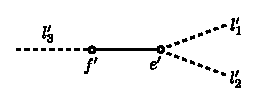
\includegraphics{figure/fig24.eps}
\end{figure}\pageoriginale

\section{Relative $n$-manifolds and their handle presentations}\label{chap8-sec8.2}

A relative $n$-manifold is a pair $(M,X)$, $X\subset M$, such that for every $a\in M-X$, the link of $a$ in $M$ is either an $(n-1)$-cell or an $(n-1)$-sphere. If $(M,X)$ is a relative $n$-manifold, $\p (M,X)$ denotes the set of points of $M-X$ whose links are cells. $\p(M,X)$ is not a polyhedron, but $\p (M,X)\cup X$ and $\overline{\p(M,X)}=\p(M,X)\cup (X\cap \overline{\p(M,X)})$ are polyhedra; so that $(\p (M,X)\cup X,X)$ and $(\overline{\p (M,X)},X')$ (where $X^{1}=X\cap \overline{\p(M,X)}$) are relative $(n-1)$-manifolds without boundary. Any compact set in $\p(M,X)$ is contained in an $(n-1)$-manifold contained in $\p(M,X)$.

We\pageoriginale sometimes denote a relative manifold $(M,X)$ by Gothic letter such as $\mathscr{M}$, and $\p (M,X)$ by $\p\mathscr{M}$.

If $(M,X)$ is a relative $n$-manifold, and $A$ an $n$-manifold, such that $A\cap M=\p A\cap \p (M,X)$ is an $(n-1)$-manifold, then it is easily proved that (using, of course, theorems on cells in spheres etc..) that $(M\cup A,X)$ is a relative $n$-manifold. As in the case of the manifolds, we have the following proposition:

\begin{proposition}\label{chap8-prop8.2.1}
Let $(M,X)$ be a relative $n$-manifold, $C$ an $n$-cell such that $C\cap M=\p C\cap \p (M,X)$ is an $(n-1)$-cell. Let $\mathscr{U}$ be any neighbourhood of $C\cap M$ in $M$. Then there is an equivalence
$$
f:(M,X)\approx (M\cup C,X)
$$
which is identity outside $\mathscr{U}$.
\end{proposition}

Let $B\subset \p A$, and $f:B\to M$ be an embedding with $f(B)\subset \p (M,X)$, and $B$ an $(n-1)$-manifold. Then there is an identification polyhedron $M\cup_{f}A$; and with the obvious convention of not distinguishing notationally between $X$ and its image in $(M\cup_{f}A)$, we have $(M\cup_{f}A,X)$ is a relative $n$-manifold, which we shall say is obtained from $(M,X)$ by {\em attaching} $(A,B)$ {\em by an embedding} $f$. Of course, doing all this rigorously involves abstract simplicial complexes, their realizations and proper abuse of notation; and we assume that this is done in each case without mention.

Let $\mathscr{M}=(M,X)$ be a relative $n$-manifold, and $\mathfrak{h}_{1},\ldots,\mathfrak{h}_{p}$ be $(n,i)$-handles, $\mathfrak{h}_{j}=(H_{j},T_{j})$. We speak of $\mathscr{M}+\mathfrak{h}_{1}+\cdots+\mathfrak{h}_{p}$, when
\begin{itemize}
\item[(1)] $H_{i}\cap H_{j}=\emptyset$

\item[(2)] $H_{i}\cap M=T_{i}\subset \p \mathscr{M}$,\pageoriginale for all $i$.
\end{itemize}

In such a case by definition,
$$
\mathscr{M}+\mathfrak{h}_{1}+\cdots+\mathfrak{h}_{p}=(M\cup H_{1}\cup\ldots\cup H_{p},X).
$$

And we say that $\mathscr{M}+\mathfrak{h}_{1}+\cdots+\mathfrak{h}_{p}$ is obtained from $\mathscr{M}$ by attaching $p(n,i)$-handles or $p$ $i$-handles.

Also if we have $f_{i}:T_{i}\to \p \mathscr{M}$ embeddings for $i=1,\ldots,p$ and $f_{i}(T_{i})\cap f_{j}(T_{j})=\emptyset$ for $i\neq j$, we may look at what we obtain from $\mathscr{M}$ by attaching $\mathfrak{h}_{1},\ldots,\mathfrak{h}_{p}$ by the maps $f_{1},\ldots,f_{p}$. The result we denote by $\mathscr{M}\cup_{f_{1}}\mathfrak{h}_{1}\cup \ldots \cup_{f_{p}}\mathfrak{h}_{p}$ and say that it is obtained from $\mathscr{M}$ by attaching $p(n,i)$-handles by imbeddings $f_{i}$.

\begin{definition}\label{chap8-defi8.2.2}
A {\em handle presentation} of a relative $n$-manifold $(M,X)$ is a $(n+2)$-tuple $\mathscr{H}=(A_{-1},\ldots,A_{n})$, of polyhedra such that,
\begin{itemize}
\item[(1)] $X\subset A_{-1}\subset\ldots\subset A_{n}=M$

\item[(2)] $A_{-1}\searrow X$

\item[(3)] $(A_{i},X)=\mathfrak{a}_{i}$ is a relative $n$-manifold for all $i$

\item[(4)] For each $i$, there exist finitely many handles of index
  $i$ \; $\mathfrak{h}^{(i)}_{1},\ldots,\break\mathfrak{h}^{(i)}_{p_{i}}$,
  such that
  $\mathfrak{a}_{i}=\mathfrak{a}_{i-1}+\mathfrak{h}^{(i)}_{1}+\cdots
  +\mathfrak{h}^{(i)}_{p_{i}}$. 
\end{itemize}

If follows from (3) and (4) that $A_{-1}$ is a neighbourhood of $X$ in $M$. $A_{-1}\searrow X$ implies that $A_{-1}\searrow N$, for some regular neighbourhood $N$ of $X$ in $M$ (see Chapter \ref{chap6}). We can even assume that $N\subset \text{int\,}_{M}A_{-1}$. Now if $B=b\mathfrak{d}_{M}N$, then $\overline{A_{-1}-N}\searrow B$, hence is a collar over\pageoriginale $B$. Thus there is an equivalence of $A_{-1}$ to $N$ which fixex $X$; that is polyhedrally $A_{-1}$ just looks like a regular neighbourhood of $X$ in $M$.
\end{definition}

Consider a relative $n$-manifold  $(M,X)$ where $M$ is a PL $n$-manifold, and $X$ a PL $(n-1)$-manifold in $M$. Such a relative manifold, we term a {\em special case}. If $(M,X)$ is a special case, and $\mathscr{H}=(A_{-1},\ldots,A_{n})$ is a handle presentation of $(M,X)$, then clearly $A_{-1}\approx X\times L$, moreover the equivalence can be assumed to carry $x$ to $(x,0)$ for $x\in X$.

\begin{theorem}\label{chap8-thm8.2.3}
Every relative manifold has a handle presentation. 
\end{theorem}

\begin{proof}
Let $\mathscr{M}=(M,X)$ be a relative $n$-manifold; let $\mathscr{P}$ be a regular presentation of $M$ with a subpresentation $\mathscr{X}$ covering $X$. With a centering $\eta$ of $\mathscr{P}$, we define the derived subdivision $d(\mathscr{P},\eta)$, and some derived subdivision $d^{2}\mathscr{P}$ of $d(\mathscr{P},\eta)$. Define 
\begin{align*}
& C^{\ast}=|St(\eta C, d^{2}\mathscr{P})|,\quad\text{for}\quad C\in \mathscr{P}\\
& A_{-1}=\cup \{C^{\ast}|C\in \mathscr{X}\}\\
& A_{k}=\cup\{C^{*}|C\in \mathscr{X},\quad\text{or}\quad C\in\mathscr{P}\quad\text{and}\quad \dim C\leq k\}.
\end{align*}

To thow that $\mathscr{H}=(A_{-1},\ldots,A_{n})$ is a handle presentation of $\mathscr{M}$, we note:
\begin{itemize}
\item[(1)] $A_{-1}=|N_{d(\mathscr{P},\eta)}(d\mathscr{X})|$ is a regular neighbourhood of $X$ in $M$.

\item[(2)] $(A_{-1},X)$ is a relative manifold. In fact, if $\mathcal{Q}$ is any subset of $\mathscr{P}$, containing $\mathscr{X}$, and $\mathcal{Q}^{\ast}$ denotes $\cup \{C^{*}|C\in \mathcal{Q}\}$, then $(\mathcal{Q}^{*},X)$ is a relative $n$-manifold.
\end{itemize}


These\pageoriginale are easily proved.

The only thing that remains to be shown is that $A_{-k}=A_{k-1}+k$-handles. The $k$-handles evidently have to be $(C^{*},C^{*}\cap \{\p C\}^{*})$, for $C\in\mathscr{P}-\mathscr{X}$ and $\dim C=k$. There are two different cases to consider, depending on whether $C$ is in the interior or boundary of $\mathscr{M}$. Any how, $C^{*}$ is an $n$-cell, since $\eta C\in M-X$ and $(M,X)$ is a relative $n$-manifold.

There is a canonical isomorphism
$$
Lk(\eta C, d^{2}\mathscr{P})\approx d(Lk(\eta C,d\mathscr{P})),
$$
which for $D<C$, takes $C^{*}\cap D^{*}$ to 
$$
D^{+}=|St(\eta D, d(Lk(\eta C,d\mathscr{P})))|.
$$

This shows that $C^{*}\cap \{\p C\}^{*}$ corresponds to
$$
N_{Lk(\eta C, d\mathscr{P})}(d\{p C\})\quad\text{in}\quad d(Lk(\eta C,d\mathscr{P})).
$$

A further fact is:
$$
Lk(\eta C, d\mathscr{P})=d\{\p C\}\ast \lambda C.
$$

Now if $C$ is an interior $k$-cell, $|\lambda C|$ is an $(n-k-1)$-sphere; and so, composing all these facts together, we get a polyhedral equivalence $f:\p (C^{*})\approx \p C\ast |\lambda C|$ which takes $C^{*}\cap \{\p C\}^{*}$ onto a regular neighbourhood of $\p C$. This directly shows that $(C^{*},C^{*}\cap \{\p C\}^{*})$ is a $k$-handle.

If $C$ is a boundary $k$-cell, then $|\lambda C|$ is an $(n-k-1)$-cell. Let $F$ be a cone on $|\lambda C|$; we then use the standard trick which makes $C^{*}$, which was the cone on $|Lk(\eta C, d^{2}\mathscr{P})|$, which is equivalent to $\p C\ast |\lambda C|$, equivalent to $C\times F$:
$$
g:C^{*}\approx C\times F,
$$\pageoriginale
in which the set $C^{*}\cap \{\p C\}^{*}$, which was mapped to $N_{d\{p C\}\ast \lambda C}(d\{\p C\})$, corresponds to
$$
g(C^{*}\cap \{\p C\}^{*})=(\p C)\times F.
$$

This shows, from our second way of looking at handles, that
$(C^{*},\break C^{*}\cap \{\p C\}^{*})$ is a $k$-handle. 

We might remark that in case (i), $C\cap \p (C^{*})$ is an attaching sphere, but that in case (ii), this lies in the boundary of the attaching tube; that is why case (ii) is somewhat more complicated than case (i).
\end{proof}

\section{Statement of the theorems, applications, comments}\label{chap8-sec8.3}

Here we state the main theorems of handle-theory and apply them to situations such as $s$-cobordism and unknotting. We outline the proofs, so that the rest of our work is devoted to the techniques which make this outline valid. We say a few words about gaps (such as a thorough discussion of Whitehead torsion)  for which there are adequate references. Our theorems and proofs are quite similar to those well-known for differential manifolds; of course, there is no worry about rounding off corners; there is no need to use isotopy-extension theorems, since cellular moves suffice. Finally, the crucial point is for homotopy to imply isotopy in certain unstable dimensions; the result needed here has been described by Weber, [see C.\@ Weber, L'\'elimination des points doubles dans le cas combinatoire, Comm.\@ Math.\@ Helv., Vol.41, Fasc 3, 1966-67]; for variety and interest, we prove the necessary result in a quite different way 

\begin{definition}\label{chap8-defi8.3.1}
A\pageoriginale relative $n$-manifold $(M,X)$ is said to be {\em geometrically trivial}, if $M\searrow X$.
\end{definition}

If $(M,X)$ is a special case, where $X$ is an $(n-1)$-submanifold of $\p M$, $M$ and $n$-manifold, when geometric triviality means just that $M\approx X\times I$ with $X$ corresponding to $X\times 0$.

When $A\subset B$ are finite CW-complexes, with $A\hookrightarrow B$ a homotopy equivalence, the {\em torsion} of $(B,A)$, denoted by $\tau(B,A)$, is a certain element of the Whitehead group of $\pi_{1}(B)$.

\begin{definition}\label{chap8-defi8.3.2}
Suppose $(M,X)$ is a special case. That $(M,X)$ is {\em algebraically trivial} means:
\begin{itemize}
\item[(1)] $X\hookrightarrow M$ is a homotopy equivalence.

\item[(2)] $\tau (M,X)=0$

\item[(3)] $\p (M,X)\hookrightarrow M$ induces an isomorphism on $\pi_{1}$.
\end{itemize}
\end{definition}

[Remark: Using a form of Lefschetz duality in the universal covering spaces, it is provable that (3) is implied by (1) plus the weaker condition that $\p (M,X)\hookrightarrow M$ induces an injection on $\pi_{1}$].

If $(M,X)$ is not a special case, let $N$ be a regular neighbourhood of $X$ in $M$. Define $M_{1}=M-N$, and $X_{1}=bd_{M}N$. Then $(M_{1},X_{1})$ is a special case, uniquely determined, upto polyhedral equivalence, by $(M,X)$. We call $(M,X)$ algebraically trivial whenever $(M_{1},X_{1})$ is algebraically trivial.

When we know of $(M,X)$ that only conditions (1) and (3) are satisfied, $(M,X)$ being special, we call $(M,X)$ an {\em $h$-cobordism}, and $\tau(M,X)$ the {\em torsion} of this $h$-cobordism.

Clearly, if $(M,X)$ is geometrically trivial, it is also algebraically\pageoriginale trivial. The converse, we shall show, is true for relative $n$-manifold, $n\geq 6$.

Let $(M,X)$ be a relative $n$-manifold which is a special case. Here are the main results.

\begin{alphtheorem}\label{chap8-thmA}
If $(M,X)$ is $1$-connected, and $\ell\leq n-4$, then $(M,X)$ has a handle presentation with no handles of indices $\leq \ell$. If furthermore, $(M,X)$ has a handle presentation with handles of indices $\leq p$ only, then it has a handle presentation with handles of indices $\geq \ell+1$ and $\leq \Max (\ell+2,p)$ only. 
\end{alphtheorem}

\begin{alphtheorem}\label{chap8-thmB}
If $(M,X)$ has a handle presentation with handles of indices $\leq n-3$ only, and $n\geq 6$, and if $X\hookrightarrow M$ is a homotopy equivalence with $\tau(M,X)=0$, then it has a presentation without any handles; so that $M\searrow X$.
\end{alphtheorem}

\begin{alphtheorem}\label{chap8-thmC}
If $(M,X)$ is algebraically trivial and $n\geq 6$, then it is geometrically trivial.
\end{alphtheorem}

Theorem \ref{chap8-thmC} holds for the general relative $n$-manifold, and this follows from Theorem \ref{chap8-thmC} in the special case by referring to the special case $(M_{1},X_{1})$ described earlier.

Theorem \ref{chap8-thmA} and \ref{chap8-thmB} imply Theorem \ref{chap8-thmC} by {\em duality}, which is described in \ref{chap8-sec8.8}. We start with a handle presentation $\mathscr{H}$ of $(M,X)$; by Theorem \ref{chap8-thmA} we can change the dual presentation $\mathscr{H}^{*}$ into one with no handles of index $\leq n-4$; dualizing this, we get a handle presentation $\mathscr{H}_{1}$ of $(M,X)$ without handles of indices $\geq 4$; since $n\geq 6$, Theorem \ref{chap8-thmB} applies to $\mathscr{H}_{1}$.

\setcounter{subsection}{2}
\subsection{}\label{chap8-sec8.3.3}
We now list the techniques used in proving Theorems \ref{chap8-thmA} and \ref{chap8-thmB}.

\medskip
(1)~ {\em Cancelling\pageoriginale pairs of handles.} In a handle presentation $\mathscr{H}=(A_{-1},\ldots,A_{n})$, sometimes there is a very explicit geometrical reason why a $(k-1)$-handle $\mathfrak{h}$ and a $k$-handle $\mathfrak{K}$ nullify each other, so that they can be dropped from the handle presentation. If $N$ is the transverse tube of $\mathfrak{h}$, and $T$ the attaching tube of $\mathfrak{K}$, and $N-N\cap T$ and $T-N\cap T$ are both $(n-1)$-cells, this is the case. This alone suffices to prove Theorem \ref{chap8-thmA} when $\ell=0$. We discuss this in \ref{chap8-sec8.5}.

\medskip
(2)~ {\em Modifying the handle presentation.} We want to shrink down transverse and attaching tubes until they become manageable, and to isotop things around. This can be done without damaging the essential structure, which consists of (a) The polyhedral equivalence class of $(M,X)$, (b) The number of handles of each index, (c) The salient features of the algebraic structure, namely, the maps $\pi_{k}(A_{k},A_{k-1})\to \pi_{k-1}(A_{k-1},A_{k-2})$ and bases of these groups. This is done in \ref{chap8-sec8.4}.

\medskip
(3) {\em Inserting cancelling pairs of handles,} the opposite to (1) is sometimes necessary in order to simplify the algebraic structure; this occurs in \ref{chap8-sec8.6}. This, together with (1) and (2), allows us to prove Theorem \ref{chap8-thmA} for $\ell=1$, at the expense of extra 3-handles. Once we have done this, there are no more knotty group-theoretic difficulties, and the universal covering spaces of the $A_{i}$'s are all embedded in each other. Then we can take a closer look at.

\medskip
(4)~ {\em The algebraic structure.} This consists of the boundary maps $\pi_{k}(A_{k},A_{k-1})\to \pi_{k-1}(A_{k-1},A_{k-1})$. When there are no $1$-handles, these groups are free modules over the fundamental-group-ring, with bases determined, upto multiplying by $\pm \pi$, by the handles. We can change\pageoriginale bases in certain prescribed ways by inserting and cancelling pairs of handles. This allows us to set up a situation where a $(k-1)$-handle and a $k$-handle {\em algebraically} cancel. We discuss this in \ref{chap8-sec8.9}. And now, both Theorems \ref{chap8-thmA} and \ref{chap8-thmB} follow if we can get algebraically cancelling handles to cancel in the real geometric sense. This amounts to getting an {\em isotopy} out of a {\em homotopy} of attaching spheres; this is, of course, the whole point; all the other techniques are a simple translation to handle presentations of the theory of simple homotopy types of J.H.C.\@ Whitehead.


\medskip
(5)~ {\em The isotopy lemma.} This is the point where all dimensional restrictions really make themselves felt. The delicate case, which applies to $(n-3)$-and $(n-4)$-handles, just barely squeaks by.

\subsection{The $s$-cobordism theorem.}\label{chap8-sec8.3.4}
 By an {\em $s$-cobordism} is meant a triple $(M;A,B)$, where $M$ is an $n$-manifold; $A$ and $B$ are disjoint $(n-1)$-submanifolds of $\p M$; $\p M-A\cup B$ is polyhedrally equivalent to $\p A\times I$ in such a way that $\p A$ corresponds to $\p A\times 0$ (and, of course, $\p B$ to $\p A\times 1$); $A\hookrightarrow M$ and $B\hookrightarrow M$ are homotopy equivalences; and $\tau(M,A)=0$.

A {\em trivial cobordism} is a triple $(M;A,B)$ equivalent to $(A\times I;A\times 0,A\times 1)$.

\begin{theorem*}
If $(M;A,B)$ is an $s$-cobordism, and $\dim M\geq 6$, then $(M;\break A,B)$
is a trivial cobordism. 
\end{theorem*}

\begin{proof}
This follows from theorem \ref{chap8-thmC}. The pair $(M,A)$ is a relative manifold, special case; and all the hypothesis of Theorem \ref{chap8-thmC} are clearly valid; in particular, $\pi_{1}(B)\approx \pi_{1}(\p M-A)\approx \pi_{1}(M)$, since $B\hookrightarrow M$ is a homotopy\pageoriginale equivalence. Hence, by theorem \ref{chap8-thmC}, $(M,A)$ is equivalent to $(A\times I,A\times 0)$. We know, by assumption, that $\overline{\p M-A\cup B}$ is a regular neighbourhood of $\p A$ in $\overline{\p M-A}$; and clearly $\p A\times I$ is a regular neighbourhood of $\p A\times 0$ in $\overline{\p (A\times I)-A\times 0}$. Thus we can fix 
up the equivalence of $(M,A)$ to $(A\times I, A\times 0)$ to take $\overline{\p M-A\cup B}$ onto $\p A\times I$; this leaves $B$ to map onto $A\times 1$, which shows the cobordism is trivial.
\end{proof}

We remark that if $\pi_{1}(A)$ is trivial, then $\tau(M,A)=0$ automatically. It is with this hypothesis that Smale originally proved his theorem; various people (Mazur and Barden) noticed that the hypothesis needed in the non-simply-connected case, was just that $A\hookrightarrow M$ he a simple homotopy equivalence (whence the ``$s$''); i.e. $\tau(M,A)=0$.

\subsection{Zeeman's unknotting theorem.}\label{chap8-sec8.3.5}
We have already described the notion of an unknotted sphere.

\begin{theorem*}
If $A\subset B$, where $A$ is a $k$-sphere, $B$ an $n$-sphere, and $k\leq n-3$, then $A$ is unknotted in $B$.
\end{theorem*}

\begin{proof}
By induction on $n$. For $n\leq 5$, the cases are all quite trivial, except for $k=2$, $n=5$, which has been treated earlier. For $n\geq 6$ we will show that the pair $(B,A)$ is equivalent to the suspension of $(B',A')$ where $B'$ is an $(n-1)$-sphere and $A'$ a $(k-1)$-sphere; and clearly the suspension of an unknotted pair of spheres is unknotted.

To desuspend, for $n\geq 6$, we proceed thus:

If $x\in A$, then the link of $x$ in $(B,A)$ is a pair of spheres which is unknotted, by the inductive hypothesis. That is to say, $A$ is {\em locally unknotted} in $B$. In particular, we can find an $n$-cell $E\subset B$,\pageoriginale such that $E\cap A$ is a $k$-cell unknotted in $E$; and so that $(\p E, \p(E\cap A))$ is bicollared in $(B,A)$; in fact, this could have been done whether or not $A$ were locally unknotted.

Define $F=\overline{B-E}$. By earlier results $F$ is an $n$-cell. Consider the relative manifold $(F,F\cap A)$. It is easily seen that this pair is algebraically trivial; because of codimension $\geq 3$ all fundamental groups are trivial, and so Whitehead torsion is no problem; the homology situation is an easy exercise in Alexander duality. Hence, by Theorem \ref{chap8-thmC}, $F$ collapses to $F\cap A$; since $F\cap A$ is a $k$-cell, it collapses to a point; putting these together, $(F,F\cap A)$ collapses to $(pt,pt)$ in the category of pairs; these collapses are homogeneous in the pair $(B,A)$ because of local unknottedness. We started with $(F,F\cap A)$ bicollared, and hence, by the regular 
neighbourhood theorem, suitably stated for pairs, $(F,F\cap A)$ is a regular neighbourhood of $x\in A$ in $(B,A)$, which is an unknotted cell pair (again using local unknottedness).

Thus $(B,A)$ is the union of two unknotted cell pairs $(E,E\cap A)$ and $(F,F\cap A)$, which shows it is polyhedrally equivalent to the suspension of $(\p E, \p (E\cap A))$.
\end{proof}

\begin{rem}\label{chap8-rem1}
This is just Zeeman's proof, except that we use our Theorem \ref{chap8-thmC} where Zeeman uses the cumbersome technique of `sunny collapsing''.
\end{rem}

\begin{rem}\label{chap8-rem2}%2
Lickorish has a theorem for desuspending general suspensions embedded in $S^{n}$ in codimension $\geq 3$. It is possible, by a similar argument, to replace ``sunny collapsing'' by Theorem \ref{chap8-thmC}. The case\pageoriginale $n=5$ can be treated by a very simple case of sunny collapsing.
\end{rem}

\begin{rem}\label{chap8-rem3}
If $A\subset B$, where $A$ is an $(n-2)$-sphere locally unknotted in the $n$-sphere $B$, and $n\geq 6$, and $B-A$ has the homotopy type of a $1$-sphere, then $A$ is unknotted in $B$.
\end{rem}

Proof exactly as in the codimension $3$ case; we need to know that Whitehead torsion is OK, which it is since the fundamental group of the $1$-sphere is infinite cyclic; and this group has zero Whitehead torsion, by a result of Graham Higman (units of group-rings).


\begin{rem}\label{chap8-rem4}%4
It has been a folk result for quite a while that the Unknotting Theorem followed from the proper statement of the $h$-cobordism theorem.
\end{rem}

\subsection{Whitehead torsion.}\label{chap8-sec8.3.6}
For any group $\pi$, there is defined a commutative group $Wh(\pi)$. Elements of $Wh(\pi)$ are represented by square, invertible matrices over the integer group ring $Z\pi$. Two matrices $A$ and $B$ represent the same element in $Wh(\pi)$, if and only if there are identity matrices $I_{k}$ and $I_{\ell}$, and a product $E$ of elementary matrices, so that $A\oplus I_{K}=E$. $(B\oplus I_{\ell})$. Here
\begin{align*}
& I_{k}\quad\text{denotes the } k\times k\text{~ identity matrix.}\\
& U\oplus V=
\begin{pmatrix}
U & 0\\
0 & V
\end{pmatrix}
\end{align*}

An elementary matrix is one of the following:
\begin{itemize}
\item[(a)] $I_{n}+e_{ij}$, where $e_{ij}$ is the $n\times n$ matrix all of whose entries are zero except for the $ij^{\text{th}}$ which is $1$; and $i\neq j$.

\item[(b)] $E_{n}(\alpha;K)$, which is the $n\times n$ matrix equal to the identity matrix, except that the $kk^{\text{th}}$ entry is $\alpha$; we restrict $\alpha$ to be an element of $\pm \pi$.
\end{itemize}

By\pageoriginale cleverly composing matrices of this sort, we can obtain $I_{n}+\lambda e_{ij}$ for any $\lambda \in Z\pi$, for instance.

Addition in $Wh(\pi)$ is induced from $\oplus$, or, equivalently, from matrix multiplication.

The geometric significance of $Wh(\pi)$ is that a homotopy equivalence $f:K\to L$ between finite $CW$-complexes determines an element of $Wh(\pi)$, $\pi=\pi_{1}(K)$, called the {\em torsion} of $f$. If the torsion is zero, wonderful things (e.g.\@ $s$-cobordism) happen.

If $\pi$ is the trivial group, then $Wh(\pi)=0$, basically because $Z\pi$ is then a Euclidean domain.

If $\pi$ is infinite cyclic, then $Wh(\pi)=0$, by Higman. His algebraic argument is easily understood; it is, in some mystical sense, the analogue of breaking something the homotopy type of a circle into two contractible pieces on which we use the result for the trivial group.

If $\pi$ has order $5$, then $Wh(\pi)\neq 0$. In fact, recent computations show $Wh(\pi)$ to be infinite cyclic.

Various facts about $Wh$ can be found in Milnor's paper. [``Whitehead Torsion'' Bulletin of A.M.S., Vol.~72, No.~3, 1966]. In particular, the torsion of an $h$-cobordism can be computed (in a straight-forward, may be obvious, way) from any handle presentation.

There is another remark about matrices that is useful. Let $A$ be an $n\times k$ matrix over $Z\pi$, such that any $k$-row-vector [i.e.\@ $1\times k$ matrix] is some left linear combination, with coefficients in $Z \pi$, of the rows of $A$; in other words, $A$ corresponds to a {\em surjection}\pageoriginale of a free $Z\pi$-module with $n$ basis elements onto one with $k$ basis elements. Let $0_{k}$ denote the $k\times k$ zero matrix. Then there is a product of elementary $(n+k)\times (n+k)$ matrices, $E$, so that $E$. $\left(\begin{smallmatrix} A\\ 0_{k}\end{smallmatrix}\right)=\left(\begin{smallmatrix}I_{k}\\ 0_{n\times k}\end{smallmatrix}\right)$. This is an easy exercise.

\subsection{}\label{chap8-sec8.3.7}
In homotopy theory we shall use such devices as univesal covering spaces, the relative Hurewicz theorem, and some homology computations (with infinite cyclic coefficient group). For example, if $(H,T)$ is a $k$-handle, then
\begin{align*}
& H_{i}(H,T)=0\quad\text{for}\quad i\neq h\\
& H_{k}(H,T)=Z,\quad \text{an infinite cyclic group,}
\end{align*}

We always arrange to have the fundamental group to act on the left on the homology of the universal covering space.

Suppose that $(M,X)$ is a relative $n$-manifold, special case, and
$(N,\break X)=(M,X)+\mathfrak{h}_{1}+\cdots+\mathfrak{h}_{p}$, where the $\mathfrak{h}$'s are handles of index $k$. Suppose $X$, $M$, $N$ are connected, and that $\pi_{1}(M)\to \pi_{1}(N)$ is an isomorphism; this implies that we can imagine not only that $M\subset N$, but that $\tilde{M}\subset \tilde{N}$, where ``$\sim$'' denotes universal covering space. Call $\pi=\pi_{1}(M)$.

Then the homology groups $H_{i}(\tilde{N},\tilde{M})$ are left $Z\pi$-modules. More explicitly, $H_{i}(\tilde{N},\tilde{M})=0$ if $i\neq k$; and $H_{k}(\tilde{N},\tilde{M})$ is a free $Z\pi$-module with basis $\{[\mathfrak{h}_{1}],\ldots,[\mathfrak{h}_{p}]\}$. What does $[\mathfrak{h}_{j}]$ mean? We take any lifting of $\mathfrak{h}_{j}=(H,T)$ to a handle $(H',T')$ in $\tilde{N}$; we pick either generator of $H_{k}(H',T')$, and map into $H_{k}(\tilde{N},\tilde{M})$ by inclusion, the result is $[\mathfrak{h}_{j}]$. The ambiguity in defining $[\mathfrak{h}_{j}]$ is simply\pageoriginale stated: If we make another choice, then instead of $[\mathfrak{h}_{j}]$ we have $\alpha[\mathfrak{h}_{j}]$, where $\alpha\in \pm \pi$.

When $k\geq 2$, we can go further and say that, by the relative Hurewicz theorem, $\pi_{k}(\tilde{N},\tilde{M})\approx H_{k}(\tilde{N},\tilde{M})\approx \pi_{k}(N,M)$. And thus we have a fairly well-defined basis of $\pi_{k}(N,M)$ as a $2\pi$-module, dependent on the handles $\mathfrak{h}_{1},\ldots,\mathfrak{h}_{p}$.

This shows, by the way, that $(N,M)$ is $(k-1)$-connected. We might have expected this, since, homotopically, $N$ is obtained from $M$ by attaching $k$-cells.

Another thing is a version of Lefschetz duality as follows: If $M$ is an oriented manifold, and $X\subset M$ with $X$ a polyhedron, then $H^{i}(M,X)\approx H_{n-i}(M,\p M-X)$. Since universal covering spaces can all be oriented, this works there. In particular, if $X\hookrightarrow M$ is a homotopy equivalence, then $H^{i}(\tilde{M},\tilde{X})=0$ for all $i$, and so $H_{i}(\tilde{M},\p \tilde{M}-\tilde{X})=0$ for all $i$. When $\p \tilde{M}-\tilde{X}$ is the universal covering space of $\p M-X$, that is, when $\pi_{1}(\p M-X)\approx \pi_{1}(M)$, then the relative Hurewicz theorem will show that $\p M-X\hookrightarrow M$ is a homotopy 
equivalence.

\subsection{Infinite polyhedra.}\label{chap8-sec8.3.8}
An {\em infinite polyhedron} $P$ is a locally compact subset of some finite-dimensional real vector space, such that for every $x\in P$, there is an ordinary polyhedron $Q\subset P$, such that $x$ is contained in the topological interior of $Q$ in $P$. A {\em polyhedral map} $f:P_{1}\to P_{2}$, between infinite polyhedra is a function, such that for every ordinary polyhedron $Q\subset P_{1}$, the graph $\Gamma(f|Q)$ is an ordinary polyhedron.

The category of infinite polyhedra includes ordinary polyhedra;\pageoriginale and in addition, every open subset of an infinite polyhedron is an infinite polyhedron.

The link of a point in an infinite polyhedron is easily defined; it turns out to be a polyhedral equivalence class of ordinary polyhedra. Hence the notions of manifold any boundary in this setting are easily defined.

If $M$ is an infinite $n$-manifold, then any compact subset $X\subset M$ is contained in the topological interior of some ordinary $n$-manifold $N\subset M$.

As for isotopies, we restrict ourselves to isotopies which are the identity outside some compact set; such are the isotopies obtained from finitely many cellular moves. Any such isotopy on the boundary of $M$ can be extended to an isotopy of this sort on $M$.

We can talk of regular neighbourhoods of ordinary (= compact) subpolyhedra in an infinite polyhedron, and the same theorems (including isotopy, in this sense) hold.

These concepts are useful here because if $(M,X)$ is a relative $n$-manifold, then $\p (M,X)$ is an infinite $n$-manifold. And now, any isotopy of $\p(M,X)$ extends to an isotopy of $M$, leaving a neighbourhood of $X$ fixed. In other words, this is convenient language for dealing with relative manifolds. This is the only situation where we shall speak of infinite polyhedra; it is, of course, obvious that infinite polyhedra can be of use in many other cases which are not discussed in these notes (in particular, in topological applications of the ``Engulfing Theorem'').

\section{Modification of handle presentations}\label{chap8-sec8.4}\pageoriginale
If $\mathscr{X}=(A_{-1},\ldots,A_{n})$ and $\mathscr{H}'=(B_{-1},\ldots,B_{n})$ are handle presentations of the relative $n$-manifolds $(M,X)$ and $(M^{1},X^{1})$ respectively, an {\em isomorphism} between $\mathscr{H}$ and $\mathscr{H}^{1}$ is a polyhedral equivalence $h:M\to N$ taking $X$ onto $X'$ and $A_{i}$ onto $B_{i}$ for all $i$. Such an isomorphism gives a $1-1$ function between handles and preserves various other structures.

Let $\mathscr{H}=(A_{-1},\ldots,A_{n})$ be a handle presentation of the relative $n$-manifold $(M,X)$ and let $f:A_{k}\to A_{k}$ be a polyhedral equivalence taking $X$ onto itself. Then by $\mathscr{H}_{f}$ is meant the handle presentation $(B_{-1},\ldots,B_{n})$ of $(M,X)$, where
\begin{align*}
& B_{i}=f(A_{i})\quad\text{for}\quad i<k\\
& B_{k}=f(A_{k})=A_{k}\\
& B_{i}=A_{i}\quad\text{for}\quad i>k.
\end{align*}

It is clear that $\mathscr{H}_{f}$ is a handle presentation of $(M,X)$, the handles of index $>k$ are equal to those of $\mathscr{H}$, while a handle of $\mathscr{H}$ of index $\leq k$ will correspond via $f$ to a handle of $\mathscr{H}_{f}$.

There is another way upto isomorphism of looking at $\mathscr{H}_{f^{-1}}$.

Suppose $f:A_{k}\to A_{k}$ is as before. Let $(H,T)$ be a $(k+1)$-handle of the presentation $\mathscr{H}$. Attach $(K,T)$ to $A_{k}$ not by the inclusion of $T$ in $\p (A_{k},X)$, but by $f|T$. In this way attaching all $(k+1)$-handels we get a relative manifold $(B_{k+1},X)$ and an equivalence $f_{k+1}$ extending $f$. Similarly attach the $(k+2)$-handles to $B_{k+1}$ one for each $(k+2)$-handle of $A_{k+2}$ by the map $f_{k+1}$ suitably restricted; and so on. In this way we get a relative manifold $(B_{n},X)$ and\pageoriginale a handle presentation $(A_{-1},\ldots, A_{k},B_{k+1},\ldots,B_{n})$ of $(B_{n},X)$. This will be denoted by $\mathscr{H}^{f}$. $f_{n}$ gives an equivalence of $(M,X)$ with $(B_{n},X)$ and an isomorphism of $\mathscr{H}_{f^{-1}}$ with $\mathscr{H}^{f}$.

The main use in this chapter of the above modifications is for simplifying handle presentations, that is to obtain presentations with as few handles as possible, or without any handles or without handles upto certain index using the given algebraic data about $(M,X)$. It should be noted that (1) $\mathscr{H}_{f}$ need not be isomorphic to $\mathscr{H}$ and (2) $\mathscr{H}^{f}$ is not a handle presentation of $(M,X)$. (2) is not a serious drawback, since $\mathscr{H}^{f}$ isomorphic to $\mathscr{H}_{f^{-1}}$ via $f^{-1}_{n}$ and so whatever simplification one can do for $\mathscr{H}^{f}$ can be done also for $\mathscr{H}_{f^{-1}}$, which  is a handle presentation of $(M,X)$ or we can first do the simplifications in $\mathscr{H}^{f}$ and pull the new handle presentation to one of $(M,X)$ by $f^{-1}_{n}$. We will adopt the procedure which is convenient in the particular case.
If $f:A_{k}\to A_{k}$ is isotopic to the identity leaving $X$ fixed, (and this will be usually the case), then $\mathscr{H}$ and $\mathscr{H}_{f}$ will have many homotopy properties in common; but more of this later.

The most frequently used ways of modifications are catalogued below:

\subsection{}\label{chap8-sec8.4.1}
Let $(H,T)$ be a $k$-handle of the presentation $\mathscr{H}=(A_{-1},\ldots,A_{n})$ of $(M,X)$. Then if $S$ is a transverse sphere and $N=\overline{\p H-T}$ the transverse tube, we have $N$ a regular neighbourhood of $S$ in $\p (A_{k},X)$. If $N'$ is any other regular neighbourhood of $S$ in $\p (A_{k},X)$, there is an isotopy of $\p (A_{k},X)$ relating $N$ and $N'$ and this can be extended to\pageoriginale $A_{k}$, to give an end result $f_{1}$, with $f_{1}(N)=N'$. Then $\mathscr{H}_{f_{1}}$ has its new handle $(f_{1}H,f_{1}T)$ whose transverse tube in $N'$.

\subsection{}\label{chap8-sec8.4.2}
Let $(H_{1},T_{1})$ be a $(k+1)$-handle of $\mathscr{H}$, with an attaching sphere $\sum$. Then $T_{1}$ is a regular neighbourhood of $\sum$ in $\p(A_{k},X)$. If $T'_{1}$ is any other regular neighbourhood of $\sum$ in $\p (A_{k},X)$ we can obtain a polyhedral equivalence $f_{2}$ of $A_{k}$ which isotopic to $1$ fixing $X$, such that $f_{2}(T_{1})=T'_{1}$. Then $\mathscr{H}^{f_{2}}$ (which is isomorphic to $\mathscr{H}_{f^{-1}_{2}}$) will have its $(k+1)$-handle corresponding to $(H_{1},T_{1})$ to have attaching tube $T'_{1}$, and handles of index $\leq k$ will be unchanged.

Combining \ref{chap8-sec8.4.1} and \ref{chap8-sec8.4.2}, we have

\setcounter{proposition}{2}
\begin{proposition}\label{chap8-prop8.4.3}
Let $\mathscr{H}=(A_{-1},\ldots,A_{n})$ be a handle presentation of the relative $n$-manifold $(M,X)$; let $\mathfrak{h}$ be a $k$-handle and $\mathfrak{K}$ a $(k+1)$-handle with a transverse sphere of $\mathfrak{h}$ being $S$ and an attaching sphere of $\mathfrak{K}$ being $\sum$. Let $N$ and $T$ be regular neighbourhoods of $S$ and $\sum$ in $\p (A_{k},X)$. Then there is a handle presentation $\mathscr{H}'$ of $(M',X')$ is equivalent to $(M,X)$ with $\mathscr{H}'$ being isomorphic to $\mathscr{H}_{f}$ for some $f:A_{k}\to A_{k}$ isotopic to the identity
leaving $X$ fixed; so that in $\mathscr{H}'$ the handles $\mathfrak{h}'$ and $\mathfrak{K}'$ corresponding to $\mathfrak{h}$ and $\mathfrak{K}$ are such that:
\begin{quote}
the transverse tube of $\mathfrak{h}'$ is $N$,

the attaching tube of $\mathfrak{K}'$ is $T$, and

the $k^{\text{th}}$ level $A'_{k}$ of $\mathscr{H}'$ is equal to the

$k^{\text{th}}$ level $A_{k}$ of $\mathscr{H}$.
\end{quote}
\end{proposition}

\begin{proof}
Using the equivalences $f_{1}$ and $f_{2}$ given by \ref{chap8-sec8.4.1} and \ref{chap8-sec8.4.2},\break $(\mathscr{H}_{f_{1}})^{f_{2}}$\pageoriginale is the required presentation. It is isomorphic to the presentation $\mathscr{H}_{(f^{-1}_{2}f_{1})}$ of $(M,X)$. Since both $f_{1}$ and $f_{2}$ are isotopic to the identity leaving $X$ fixed, $f^{-1}_{2}f_{1}$ has the same property. The last point is obvious.
\end{proof}

\setcounter{subsection}{3}
\subsection{}\label{chap8-sec8.4.4}
Let $\mathfrak{K}=(H,T)$ be a $(k+1)$-handle of $\mathscr{H}$, and $S$ an attaching sphere of $\mathfrak{K}$. $S$ is in $\p (A_{k},X)$. Suppose that $S'$ is another $k$-sphere in $\p (A_{k},X)$ and that there is an equivalence $f$ of $A_{k}$ taking $X$ onto itself and such that $f(S)=S^{1}$. Then in $\mathscr{H}^{f}$, the handle $\mathfrak{K}^{1}$ corresponding to $\mathfrak{K}$ will have $S^{1}$ as an attaching sphere. If, for example, we can go from $S$ to $S^{1}$ by cellular moves, the we can obtain an equivalence $f$ of $A_{k}$ isotopic to $1$ leaving
$X$ fixed and with $f(S)=S^{1}$. This will also be used in cancellation of handles, where it is more convenient to have certain spheres as attaching spheres than the given ones.

\subsection{}\label{chap8-sec8.4.5}
Let $\mathfrak{h}$ be a $k$-handle in a handle presentation $\mathscr{H}=(A_{-1},\ldots,A_{n})$ of a relative $n$-manifold. Then if $k\leq n-2$, there is $h$ isotopic to the identity, $h:A_{k}\to A_{k}$, leaving $X$ fixed, such that the handle $\mathfrak{h}^{1}$ of $\mathscr{H}_{h}$ corresponding to $\mathfrak{h}$ has a boundary core in $\p(A'_{k+1},X)$ where $\mathscr{H}_{h}=(A'_{-1},\ldots,A'_{n})$.

(Reader, have faith that this is usefull)

We prove this by choosing attaching spheres for all the $(k+1)$-handles, finding a transverse sphere for $\mathfrak{h}$ that intersects all the attaching spheres only finitely, noting that the transverse sphere contains other points, and then shrinking the attaching tubes and the transverse\pageoriginale tube conveniently. More explicitly.

Let $\mathfrak{K}_{1},\ldots,\mathfrak{K}_{p}$ be the $(k-1)$-handles of $\mathscr{H}$, with attaching spheres $S_{1},\ldots,S_{p}$. Let $N$ be the transverse tube of $\mathfrak{h}$; there is a polyhedral equivalence $f:N\approx D^{k}\times \Delta^{n-k}$, so that for any $x\in \text{int\,}D^{k}$, $f^{-1}(k\times \p \Delta^{n-k})$ is a transverse sphere to $\mathfrak{h}h$. Now, $(S_{1}\cup\ldots\cup S_{p})\cap N$ is $(\leq k)$-dimensional, and so, triangulating proj$_{D}k\cdot f$ so as to be simplicial and picking $x$ in the interior of a $k$-simplex of $D^{k}$ (see  \ref{chap4-coro4.2.14}), we have found a transverse sphere $\sum =f^{-1}(x\times \p \Delta^{n-k})$ to $\mathfrak{h}$, such that $\sum \cap (S_{1}\cup \ldots \cup S_{p})$ is finite. Now, $\sum$ is an $(n-k-1)$-sphere; and since $k\leq n-2$, contains infinitely many points; there is $y\in \sum-(S_{1}\cup\ldots,\cup S_{p})$. 

Now then, if we take very thin regular neighbourhoods of $\sum$, $S_{1},\break\ldots,S_{p}$ in $\p (A_{k},X)$ the regular neighbourhood of $\sum$ will intersect those of $S_{1},\ldots,S_{p}$ in only small cells near each point of intersection of $\sum \cap (S_{1},\break\ldots,S_{p})$, and hence there will be a cross-section of the $\sum$-neighbourhood [i.e., corresponding to $D^{k}\times z$, $z\in \p \Delta^{n-k},(x,z)=f(y)$], through $y$, not meeting any of the $S_{i}$ neighbourhoods. We make these regular neighbourhoods the transverse tube of $\mathfrak{h}$ and the attaching tubes of $\mathfrak{K}_{1},\ldots,\mathfrak{K}_{p}$, by changing $\mathscr{H}$ to $(\mathscr{H}_{g_{1}})^{g_{2}}$, where $g_{1}$ and $g_{2}$ are equivalences $A_{k}\to A_{k}$ isotopic to the identity, fixing $X$. In $(\mathscr{H}_{g_{1}})^{g_{2}}$ we have a boundary core of the handle corresponding to $\mathfrak{h}$ which misses all the attaching tubes of the $(k+1)$-handles (this is that ``cross-section through $y$''). We define $h=g_{2}^{-1}g_{1}$: and since $\mathscr{H}_{h}$ is isomorphic to $(\mathscr{H}_{g_{1}})^{g_{2}}$, we have some boundary core of $\mathfrak{h}^1$ when $\mathfrak{h}^1$ is the\pageoriginale handle corresponding to $\mathfrak{h}$ which does not intersect the attaching tubes of all the $(k+1)$-handles, and is therefore in $\p (A'_{k+1},X)$.

\section{Cancellation of handles}\label{chap8-sec8.5}

\noindent
{\bf Convention:}~ Let us make the convention that a submanifold of another manifold should mean this:

If $A\subset B$, $A$ and $B$ are PL-manifolds, we call $A$ a submanifold of $B$, if and only if, $A\cap \p B$ is $(\dim A-1)$-submanifold of $\p A$. We are usually in this section interested only in the case $\dim A=\dim B$.

With this convention, if $A$ is a submanifold of $B$, then $\overline{B-A}$ is a submanifold of $B$, and $bd_{B}(A)=bd_{B}(\overline{B-A})=\overline{\p A-\p B}$. If $C\subset B\subset A$ all PL-manifolds such that each is a submanifold of the next, then $\overline{A-(\overline{B-C})}=\overline{A-B}\cup C$. We may therefore be justified somewhat in writing $A-B$ for $\overline{A-B}$.

Thus, hereafter, $A$ is a submanifold of $B$ means that $A$ is a submanifold of $B$ in the above sense, and in that case $B-A$ stands for $\overline{B-A}$.

Let $\mathscr{H}=(A_{-1},\ldots,A_{n})$ be a handle presentation of a relative $n$-manifold $(M,X)$. Let $\mathfrak{h}=(H,\p H-N)$ be a $k$-handle with transverse tube $N$, and $\mathfrak{K}=(K,T)$ be a $(k+1)$-handle with attaching tube $T$. Note that $N\cup T\subset \p (A_{k},X)$ with the above conventions we can write
$$
A_{k}+\mathfrak{h}=((A_{k}-\mathfrak{h})\cup K)\cup H.
$$

\newpage

\begin{figure}[H]
\centering
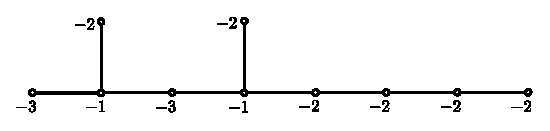
\includegraphics{figure/fig25.eps}
\end{figure}\pageoriginale 

\begin{definition}\label{chap8-defi8.5.1}
We\pageoriginale say that $\mathfrak{h}$ and $\mathfrak{K}$ can be {\em cancelled} if
\begin{itemize}
\item[(1)] $N\cap T$ is a submanifold of both $N$ and $T$

\item[(2)] $N-(N\cap T)$ and $T-(N\cap T)$ are both $(n-1)$-cells.
\end{itemize}

Suppose $\mathfrak{h}$ and $\mathfrak{K}$ can be cancelled. Then
\medskip

\noindent
{\bf Assertion 1.}~$(A_{k}-\mathfrak{h})\cap K$ is an $(n-1)$-cell contained in $\p (A_{k}-\mathfrak{h},X)$ and in $\p K$.

In fact, $(A_{k}-\mathfrak{h})\cap K=T-(N\cap T)$, which we assumed to be an $(n-1)$-cell.

\medskip
\noindent
{\bf Assertion 2.}~$((A_{k}-\mathfrak{h})\cup K)\cap H$ is an $(n-1)$-cell contained in $\p((A_{k}-\mathfrak{h})\cup K,X)$ and in $\p H$. For
\begin{align*}
((A_{k}-\mathfrak{h})\cup K)\cap H &= \text{attaching tube of } \mathfrak{h} \text{~ plus~ } N\cap T\\
&= (\p H-N)\cup (N\cap T)\\
&= \p H-(N-N\cap T)
\end{align*}
and this is an $(n-1)$-cell, since $\p H$ is an $(n-1)$-sphere and $(N-N\cap T)$ is an $(n-1)$-cell in $\p H$.
\end{definition}

Combining these two assertions with proposition \ref{chap8-prop8.2.1}, we have

\begin{proposition}\label{chap8-prop8.5.2}
Suppose $\mathscr{H}=(A_{-1},\ldots,A_{n})$ is a handle presentation of a relative $n$-manifold $(M,X)$; and there are $\mathfrak{h}=(H,\p H-N)$ a $k$-handle, and $\mathfrak{K}=(K,T)$ a $(k+1)$-handle that can be cancelled. Let $\mathscr{U}$ be any neighbourhood of $N\cap T$ in $A_{k}$. Then there is a polyhedral equivalence
$$
f:(A_{k}-\mathfrak{h},X)\approx (A_{k}+\mathfrak{K},X)
$$
which is identity outside $\mathscr{U}$.
\end{proposition}

This being so, we construct a new-handle presentation $(B_{-1},\ldots,B_{n})$\pageoriginale of $(M,X)$, which we denote by $\mathscr{H}-(\mathfrak{h},\mathfrak{K})$ as follows:
\begin{align*}
& B_{i}=f(A_{i})\quad\text{for}\quad i<k\\
& B_{k}=f(A_{k}-\mathfrak{h})=A_{k}+\mathfrak{K}\\
& B_{i}=A_{i}\quad\text{for}\quad i>k.
\end{align*}

This of course depends on $f$ somewhat observe that, since the attaching tubes of the $(k+1)$-handles are disjoint, the attaching tubes of $(k+1)$-handles other than $\mathfrak{K}$ are in $\p(A_{k},X)-T\subset \p (A_{k}+\mathfrak{K},x)$, so that $\mathscr{H}-(\mathfrak{h},\mathfrak{K})$ is a genuine handle-presentation.

\setcounter{subsection}{2}
\subsection{}\label{chap8-sec8.5.3}
(Description of $\mathscr{H}-(\mathfrak{h},\mathfrak{K})$). The number of $i$-handles in $\mathscr{H}-(\mathfrak{h},\mathfrak{K})$ is the same as the number of $i$-handles of $\mathscr{H}$ for $i\neq k$, $k+1$. For $i>k$, each $i$-handle of $\mathscr{H}$ is a $i$-handle of $\mathscr{H}-(\mathfrak{h},\mathfrak{K})$ with the single exception of $\mathfrak{K}$; and conversely. For $i\leq k$, each $i$-handle of $\mathscr{H}$ except $\mathfrak{h}$, say $\ell$, corresponds to the $i$-handle $f(\ell)$ of $\mathscr{H}-(\mathfrak{h},\mathfrak{K})$ and conversely each $i$-handle of $\mathscr{H}-(\mathfrak{h},\mathfrak{K})$ is of this form. If the attaching tube of $\mathfrak{K}$ does not interset some $k$-handle $\ell$, we can arrange $f|\ell$ to be identity, so that $\ell$ itself occurs in 
$\mathscr{H}-(\mathfrak{h},\mathfrak{K})$.

The conditions for $\mathfrak{h}$ and $\mathfrak{K}$ to cancel are somewhat stringent. We now proceed to obtain a sufficient condition on $\mathfrak{h}$ and $\mathfrak{K}$, which will enable us to cancel the handles corresponding to $\mathfrak{h}$ and $\mathfrak{K}$ in some $\mathscr{H}_{f}$. This requires some preliminaries.

Suppose $A$, $B$, $C$ are three PL-manifolds, $A\cup B\subset C-\p C$. $\dim A=p$, $\dim B=q$ and $\dim C=p+q$, $\p A=\p B=\emptyset$. Let $x\in A\cap B$. 

\setcounter{proposition}{3}
\begin{definition}\label{chap8-defi8.5.4}
$A$\pageoriginale and $B$ are said to intersect {\em transversally at $x$ in $C$}, if there is a neighbourhood $F$ of $x$ in $C$ and a polyhedral equivalence $f:F\xrightarrow{\approx}S\ast \sum \ast v$ where $S$ is a $(p-1)$-sphere, $\sum a(q-1)$-sphere, such that
\begin{itemize}
\item[(1)] $f(x)=v$

\item[(2)] $f(A\cap F)=S\ast v$

\item[(3)] $f(B\cap F)=\sum \ast v$.
\end{itemize}
\end{definition}

\begin{proposition}\label{chap8-prop8.5.5}
Let $S$ and $\sum$ be $(p-1)$-and $(q-1)$-spheres respectively and $E=S\ast \sum \ast v$. Let $D=S\ast v$, $\Delta=\sum \ast v$. Suppose $\mathscr{E}$ is any simplicial presentation of $E$ containing full subpresentations $\mathscr{D}$ and $\mathscr{A}$ covering $D$ and $\Delta$. Let $P=|N_{\mathscr{E}}(\mathscr{D})|$ and $Q=|N_{\mathscr{E}}(\mathscr{A})|$. Then 
\begin{itemize}
\item[(1)] $P\cap Q$ is a submanifold both of $P$ and $Q$ and is contained in the interior of $E$ ($P,Q$ and $P\cap Q$ are all $(p+q)$-manifolds)

\item[(2)] $P-P\cap Q\searrow P\cap \p E$

$Q-P\cap Q\searrow Q\cap \p E$.
\end{itemize}
\end{proposition}

\begin{proof}
First observe that, if the proposition is true for some centering of $\mathscr{E}$, then it is true for any centering of $\mathscr{E}$. Next, if $\mathscr{E}'$ is some other presentation of $E$ such that $D$ and $\Delta$ are covered by full subpresentations, it is possible to choose centerings of $\mathscr{E}$ and $\mathscr{E}'$ so that $P=P'$ and $Q=Q'$. ($P'$, $Q'$ denoting the analogoues of $P$ and $Q$ with reference to $\mathscr{E}'$). Thus it is enough to prove the proposition for some suitable presentation $\mathscr{E}'$ of $E$ and a suitable centering of $\mathscr{E}'$. Now we choose $\mathscr{E}'$ to be a join presentation of $E=S\ast \sum \ast v$\pageoriginale and choose the centering so that (see \ref{chap6-prop6.8.3} and the remark thereafter)
\begin{align*}
& P'Q'=|St(v,d\mathscr{E}')|=C_{\frac{1}{2}}(S\ast \sum),\\
& P'-P'\cap Q'=(P'\cap \p E)\times [\frac{1}{2},1],\quad\text{and}\\
& Q'-P'\cap Q'=(Q'\cap \p E)\times [\frac{1}{2},1].
\end{align*}

And in this case (1) and (2) are obvious.
\end{proof}

\begin{proposition}\label{chap8-prop8.5.6}
Suppose $A$ and $B$ are spheres of dimensions $p$ and $q$ respectively, contained in the interior of a $(p+q)$-manifold $C$ and that $A$ and $B$ intersect at a single point $x$ transversally in $C$. Then there are regular neighbourhoods $N$ and $T$ of $A$ and $B$ in $C$, such that
\begin{itemize}
\item[(1)] $N\cap T$ is a submanifold of both $N$ and $T$

\item[(2)] $N-(N\cap T)$ and $T-(N\cap T)$ are both $(p+q)$-cells.
\end{itemize}
\end{proposition}

\begin{proof}
Let $F$ be the nice neighbourhood of $x$ in $C$ given by \ref{chap8-defi8.5.4} i.e.\@ there is a polyhedral equivalence $f:F\approx E=S\ast \sum\ast v$ where $S$ is a $(p-1)$-sphere and $\sum$ a $(q-1)$-sphere, such that $f(x)=v$, $f(A\cap F)=S\ast v$, and $f(B\cap F)=\sum\ast v$. Then $(\overline{A-F})$ is a $(p-1)$-cell and $(\overline{B-F})$ is a $(q-1)$-cell. Let $\mathscr{S}_{1}$ and $\mathscr{E}_{1}$ be triangulations of $F$ and $E$ such that $f$ is simplicial with reference to $\mathscr{S}_{1}$ and $\mathscr{E}_{1}$. We can assume $\mathscr{E}_{1}$ contains full subpresentations covering $S\ast v$ and $\sum \ast v$. Now some 
refinement $\mathscr{S}$ of $\mathscr{S}_{1}$ can be extended to a neighbourhood of $A\cup B$, denote it by $\mathscr{S}'$, it can be supposed that $\mathscr{S}'$ contains full subpresentations $\mathfrak{a}$, $\mathscr{B}$ covering $A$, $B$ respectively. Let $\eta$ be a centering of $\mathscr{S}'$. Denote\pageoriginale by $\mathscr{E}$ the triangulation of $E$ corresponding to $\mathscr{S}$ by $f$, and by $\mathfrak{b}$ the centering of $\mathscr{E}$ corresponding to $\eta|\mathscr{S}$. Choose $N=|N_{\mathscr{S}'}(\mathfrak{a})|$ and $T=|N_{\mathscr{S}'}(\mathscr{B})|$; and let $P$, $Q$ be as in \ref{chap8-prop8.5.5}. If $P_{1}=f^{-1}(P)$, $Q_{1}=f^{-1}(Q)$, then $P_{1}=(P_{1}\cap Q_{1})\searrow P_{1}\cap\p F$ and $Q_{1}-(P_{1}\cap Q_{1})\searrow Q_{1}\cap \p F$. Clearly $P_{1}\subset N$, $Q_{1}\subset T$ are submanifolds and $N\cap T=P_{1}\cap Q_{1}$. Thus $N\cap T$ is a submanifold of both $N$ and $T$. $N-(N\cap T)=N-(P_{1}\cap Q_{1})=(N-P_{1})\cup (P_{1}-(P_{1}\cap Q_{1}))$ collapses to $(N-P_{1})$ since $P_{1}-(P_{1}\cap Q_{1})$ collapses
$P_{1}\cap\p F\subset (N-P_{1})$. But $N-P_{1}$ is a regular neighbourhood of $\overline{A-F}$ in $C-F$ which is a $(p-1)$-cell. Thus $N-(N\cap T)\searrow N-P_{1}\searrow \overline{A-F}$ which is collapsible. Thus $N-(N\cap T)$ is a collapsible $(p+q)$-manifold, hence a $(p+q)$-cell. Similarly $T-(N\cap T)$ is a $(p+q)$-cell. 
\end{proof}

\begin{definition}\label{chap8-defi8.5.6}
Let $\mathscr{H}=(A_{-1},\ldots,A_{n})$ be a handle presentation of a relative $n$-manifold $(M,X)$. Let $\mathfrak{h}$ be a $k$-handle and $\mathfrak{K}$ be a $(k+1)$-handle of $\mathscr{H}$. We say that $(\mathfrak{h},\mathfrak{K})$ {\em can be nearly cancelled} if there is a transverse sphere $S$ of $\mathfrak{h}$ and an attaching sphere $\sum$ of $\mathfrak{K}$ which intersect a single point transversally in $\p (A_{k},X)$.
\end{definition}

\begin{proposition}\label{chap8-prop8.5.7}
Suppose $\mathscr{H}$ is a handle presentation of relative $n$-manifold $(M,X)$, $\mathfrak{h}$ a $k$-handle and $\mathfrak{K}$ a $(k+1)$-handle in $\mathscr{H}$. If $\mathfrak{h}$ and $\mathfrak{K}$ can be nearly cancelled, then there is a polyhedral equivalence $f:A_{k}\to A_{k}$ isotopic to the identity leaving $X$ fixed such that, in $\mathscr{H}_{f}$ the handles $\mathfrak{h}'$ and $\mathfrak{K}'(=\mathfrak{K})$ corresponding to $\mathfrak{h}$ and $\mathfrak{K}$ can be cancelled.
\end{proposition}

\begin{proof}
Follows from \ref{chap8-prop8.4.3} and \ref{chap8-prop8.5.6}.
\end{proof}

\section{Insertion of cancelling pairs of handles}\label{chap8-sec8.6}\pageoriginale

In this section we discuss the insertion of cancelling pairs of handles and two applications which are used in the following sections. First we form a standard trivial pair as follows:
\begin{figure}[H]
\centering
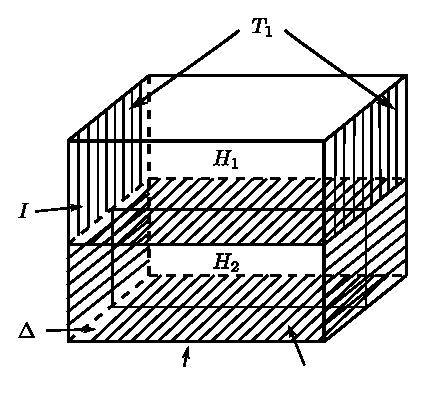
\includegraphics{figure/fig26.eps}
\end{figure}

Let $D$ be a $k$-cell, $I=[0,1]$ and $\Delta$ an $(n-k-1)$-cell. Then $E=D\times I\times \Delta$ is an $n$-cell. Let
\begin{align*}
H_{1} &= D\times [\frac{1}{2},1]\times \Delta\\
T_{1} &= \p D\times[\frac{1}{2},1]\times \Delta
\end{align*}

Clearly $\mathfrak{h}=(H_{1},T_{1})$ is a handle of index $k$. Next, let
\begin{align*}
H_{2} &= D\times [0,\frac{1}{2}]\times \Delta\\
T_{2} &= \p \{D\times [0,\frac{1}{2}]\}\times D\\
&= \{(D\times 0)\cup (D\times \frac{1}{2})\cup (\p D\times [0,\frac{1}{2}])\}\times \Delta.
\end{align*}

Clearly, $\mathfrak{K}=(H_{2},T_{2})$ is a handle of index $(k+1)$. Finally, let $F$ denote $(D\times 0\times \Delta)\cup (\p D\times I\times \Delta)$. $(D\times 0\times \Delta)\cap (\p D\times I\times \Delta)=\p D\times 0\times \Delta$ is\pageoriginale an $(n-2)$-manifold, hence $F$ is an $(n-1)$-manifold. Moreover $F$ is collapsible, hence it is an $(n-1)$-cell.

Now, let $\mathscr{H}$ be a handle presentation of a relative $n$-manifold $(M,X)$; we take an $(n-1)$-cell $F'$ in $\p(A_{k},X)$ away from the $k$-and $(k+1)$-handles. That is $F'$ is in the common portion of $\p(A_{k-1},X)$, $\p(A_{k},X)$ and $\p(A_{k+1},X)$ and clearly it is possible to choose such an $F'$ if $(k+1)<n$, that is $k\leq n-2$. Now we take some equivalence $\alpha:F\approx F'$ and attach $E$ to $A_{k}$ by $\alpha$. Denote the result by $A_{k}\cup E$. Since $E$ is an $n$-cell meeting $\p(A_{k},X)$ in an $(n-1)$-cell $F'$, there is an equivalence $f:A_{k}\approx A_{k}\cup E$ leaving $X$ fixed. Then we get a new handles presentation $(B_{-1},\ldots,B_{n})$ of $(M,X)$ as follows:
\begin{align*}
B_{i} &= f^{-1}(A_{i}),\quad\text{for}\quad i<k,\\
B_{k} &= f^{-1}(A_{k}+\mathfrak{h})\\
B_{i} &= A_{i}\quad \text{for}\quad i>k.
\end{align*}

Next we consider the problem of attaching a cancelling pair of $k$- and $(k+1)$-handles $(\mathfrak{h},\mathfrak{K})$ to $A_{k}$, with $\mathfrak{h}$ having a prescribed attaching sphere. We recall from Chapter \ref{chap7} (\ref{chap7-sec7.2}) that a sphere in the interior of a PL-manifold $N$ is unknotted (by definition) if it bounds a $k$-cell. In such a case it bounds an unknotted cell (again in the sense of \ref{chap7-sec7.2}). If $S$ and $S'$ are two unknotted $k$-spheres in the same component of $N-\p N$, then there is an isotopy $h_{t}$ of $N$ leaving $N$ fixed such that $h_{1}(S)=S'$. Similarly if $D$ and $D'$ are two unknotted $k$-cells in the same component of $N-\p N$, there is an isotopy of $N$ taking $D$ onto $D'$. Similar remarks apply in the case\pageoriginale of relative
manifolds also.

Now consider just $A_{k}$, let $F'$ be any $(n-1)$-cell in $\p (A_{k},X)$ and form  $A_{k}\cup E$ by an equivalence $\beta:F\approx F'$. Consider $S=\p D\times \alpha \times e$, where $\frac{1}{2}<\alpha<1$ and $e\in \Delta -\p \Delta$. $S$ is an attaching sphere of $\mathfrak{h}$, and $\sum =\p\{D\times[0,\frac{1}{2}]\}\times e$
$$
=\{(D\times 0)\cup (D\times \frac{1}{2})\cup \p D\times [0,\frac{1}{2}]\}\times e
$$
is an attaching sphere of $\mathfrak{K}$.
\begin{figure}[H]
\centering
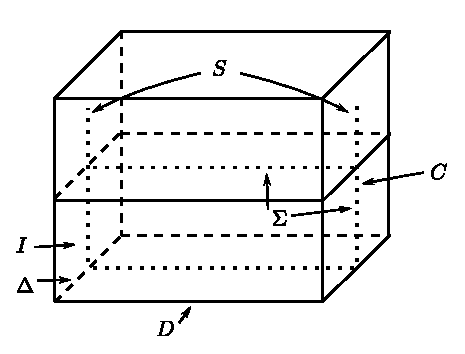
\includegraphics{figure/fig27.eps}
\end{figure}

And $\{D\times 0\cup \p D\times[0,\alpha]\}\times e=C$, say, is a $k$-cell bounding $S=\p D\times \alpha\times e$, an attaching sphere of $\mathfrak{h}$. Moreover
\begin{align*}
C\cap\sum &= \{D\times 0\cup \p D\times [0,\frac{1}{2}]\}\times e\\
&= C-\p D\times [\frac{1}{2},\alpha]\times e\\
&= C-(\text{a regular neighbourhood of $S$ in $C$}).
\end{align*}

Finally $C$ is unknotted in $F$.

The result of all this is, if $A$ is a $(k-1)$-sphere bounding an unknotted $k$-cell $B$ in $\p(A_{k},X)$, then we can attach a cancelling pair\pageoriginale of $k$- and $(k+1)$-handles $(\mathfrak{h},\mathfrak{K})$ such that $A$ is an attaching sphere of $\mathfrak{h}$ and an attaching sphere of $\mathfrak{K}$ intersects $\p(A_{k},X)$ in $B$ - (a given a regular neighbourhood of $A$ in $B$). This can also be seen as follows:

Let $L$ be an $(n-1)$-cell, $A$ a $(k-1)$-sphere in $L$ bounding an unknotted $k$-cell $B$ in the interior of $L$. Let $M$ be an $n$-cell containing $L$ in its boundary. We may join $A$ and $B$ to an interior point $v$ of $M$ and take second derived neighbourhoods. Let $H$ be a second derived neighbourhood of $A\ast v$ and $K$ be the closure of [second derived neighbourhood of $B\ast v-H$]. Then $
(H,H\cap L)$ is a $k$-handle, and $(K,(K\cap H)\cup (K\cap L))$ is a $(k+1)$-handle. The $k$-handle has $A$ as an attaching sphere, and an attaching sphere of the $(k+1)$-handle intersects $L$ in ($B$ - a regular neighbourhood of $A$ in $B$). Thus we have,

\subsection{}\label{chap8-sec8.6.1}
Let $\mathscr{H}=(A_{-1},\ldots,A_{n})$ be a handle presentation of a relative $n$-manifold $(M,X)$ and let $S\subset \p (A_{k},X)$ be a $(k-1)$-sphere which bounds an unknotted cell $T$ in $\p(A_{k},X)$. Then there are a $k$-handle $\mathfrak{h}$ and a $(k+1)$-handle $\mathfrak{K}$, such that
\begin{enumerate}
\renewcommand{\labelenumi}{(\theenumi)}
\item $S$ is an attaching sphere of $\mathfrak{h}$

\item There is an attaching sphere $\sum$ of $\mathfrak{K}$ with $\sum \cap A_{k}$ very closed to $T$, that is $\sum \cap A_{k}$ can be assumed to be ($T$ - a prescribed regular neighbourhood of $S$ in $T$).

\item $((A_{k},X)+\mathfrak{h})+\mathfrak{K}$ exists and is polyhedrally equivalent to $(A_{k},X)$ by an equivalent which is\pageoriginale identity outside a given neighbourhood of $T$ in $A_{k}$.
\end{enumerate}

If $S$ is in $\p(A_{k-1},X)\cap \p (A_{k},X)$ we can choose $\mathfrak{h}$ to have its attaching tube in $\p(A_{k-1},X)$, so that there is an obvious handle presentation of $((A_{k}+\mathfrak{h})+\mathfrak{K},X)$. We give below two applications of this construction.

\subsection{Trading handles.}\label{chap8-sec8.6.2}
Let $\mathscr{H}=(A_{-1},\ldots,A_{n})$ be a handle presentation of a relative $n$-manifold $(M,X)$. Let $p_{i}$ be the number of $i$-handles in $\mathscr{H}$. Suppose that there is a $(k-1)$-handle $\ell$ $(2\leq k\leq n-1)$ with a transverse sphere $\sum$, and that there is a $(k-1)$-sphere $S$ in $\p(A_{k-1},X)\cap \p (A_{k},X)$ such that (1) $S$ is unknotted in $\p(A_{k},X)$, (2) $S$ intersects $\sum$ transversally at exactly one point in $\p(A_{k-1},X)$. Then there is a procedure by which we can obtain another handle presentation $\mathscr{H}'$ of $(M,X)$, such that (a) for $i\neq k-1$ or $k+1$, the number of $i$-handles in $\mathscr{H}$ is equal to the number of $i$-handles in $\mathscr{H}'$, (b) the number of $(k-1)$-handles in $\mathscr{H}'$ is $p_{(k-1)}-1$ (c) the number of $(k+1)$-handles in $\mathscr{H}'$ is $p_{(k+1)}+1$. This is done as follows:

First consider only $A_{k}$. Applying \ref{chap8-sec8.6.1}, we can add to $A_{k}$ a cancelling pair of $k$- and $(k+1)$-handles $(\mathfrak{h},\mathfrak{K})$ such that $S$ is an attaching sphere of $\mathfrak{h}$, and the attaching tube of $S$ is in $\p(A_{k-1},X)$. Write $(A_{k}+\mathfrak{h})+\mathfrak{K}=B$. Then the relative manifold $(B,X)$ has the obvious handle presentation $\mathscr{K}'=(B_{-1},\ldots,B_{k+1})$ where 
\begin{align*}
& B_{i}=A_{i},\quad\text{for}\quad i\leq k-1\\
& B_{k}=A_{k}+\mathfrak{h}\\
& B_{k+1}=(A_{k}+\mathfrak{h})+\mathfrak{K}=B.
\end{align*}\pageoriginale

In $\mathfrak{K}'$, the handles $\ell$ and $\mathfrak{h}$ can be nearly cancelled. Hence for some equivalence $f$ of $A_{k-1}$, isotopic to identity and leaving $X$ fixed, in $\mathscr{K}'_{f}$, the handles $\ell'$ and $\mathfrak{h}'(=\mathfrak{h})$ corresponding to $\ell$ and $\mathfrak{h}$ can be cancelled. Let $\mathscr{K}''=\mathscr{K}'_{f}-(\mathfrak{h}',\ell')$. $\mathscr{K}''$ is a handle presentation of $(B,X)$; the number of $i$-handle in $\mathscr{K}''$ for $i\leq k-1$ is $p_{i}$, the number of $(k-1)$-handles is $\mathscr{K}''$ is $p_{k-1}-1$, the number of $k$-handles is $p_{k}$ and there is one $(k+1)$-handle. Also there is an equivalence $\alpha:A_{k}\to B$ which can be assumed to be identity near $X$. Thus we can pull back $\mathscr{K}''$ to a handle presentation $\mathscr{K}$ of $(A_{k},X)$ by $\alpha^{-1}$.

Now, we would like to add the $(\geq k+1)$-handles of $\mathscr{H}$ to $\mathscr{K}$ to get a new handle presentation of $(M,X)$. But it may happen that the attaching tubes of the $(k+1)$-handles of $\mathscr{H}$ intersect the transverse tube of $\alpha^{-1}(\mathfrak{K})$ which is in $\p(A_{k},X)$. However, we can adopt the procedure of \ref{chap8-sec8.4.5}, to get the desired type of handle presentations as follows:

Let $\mathfrak{K}^{(k+1)}_{1}$, $\mathfrak{K}_{2}^{(k+1)}$, $\mathfrak{K}^{(k+1)}_{p_{(k+1)}}$ be the $(k+1)$-handles of $\mathscr{H}$, with attaching tubes $T_{1},T_{2},\ldots,T_{p_{(k+1)}}$ respectively. Choose some attaching spheres $S_{1},\ldots,S_{p_{(k+1)}}$ of these handles, and then a transverse sphere $\sum$, of $\alpha^{-1}(\mathfrak{K})$ avoiding $S_{1},\ldots,S_{p_{(k+1)}}$. This is done in the same way as in \ref{chap8-sec8.4.5}, using the\pageoriginale product structure of the transverse tube of $\alpha^{-1}(\mathfrak{K})$ as $D^{k+1}\times \Delta^{n-k-1}$ and noticing that the $S_{i}$ are now $k$-dimensional. Then choose a regular neighbourhood $N_{1}$ of $\sum_{1}$ which does not intersect the $S_{i}$'s and do a modification of type \ref{chap8-sec8.4.1} so that, for some $g$, in $\mathscr{K}_{g}$ the handle $\mathfrak{K}'$ corresponding $\alpha^{-1}(\mathfrak{K})$ has $N_{1}$ as its transverse tube. Now choose regular neighbourhoods $T'_{i}$ of $S_{i}$ in $\p (A_{k},X)$ such that $T'_{i}\cap N_{1}=\emptyset$ for all $i$ and $T'_{i}
\cap T'_{j}=\emptyset$ for all $i$, $j$, $i\neq j$. There is an equivalence $\beta$ of $A_{k}$ isotopic to the identity leaving $X$ fixed such that $\beta(T_{i})=T'_{i}$ for all $i$. Now attach the handles $\mathfrak{K}^{(k+1)}_{i}$ to $A_{k}$ not by the inclusion of $T_{i}$ but by $\beta|T_{i}$. Then we obtain a relative $n$-manifold say $(C,X)$ and a genuine handle presentation say $\mathscr{K}_{1}$ of $(C,X)$. Moreover the equivalence $\beta$ of $A_{k}$ can be extended to an equivalence $\beta_{k+1}$ of $A_{k+1}$ with $C$. Now pull back $\mathscr{K}_{1}$ to $A_{k+1}$ by $(\beta_{k+1})^{-1}$. In the handle presentation $(\beta_{k+1})^{-1}
(\mathscr{K}_{1})$ of $A_{k+1}$ there are handles only upto index $(k+1)$; so that the handle of index $\geq k+2$ of $\mathscr{H}$ can be added as they are to get a handle presentation of $(M,X)$ of the derived type.

\setcounter{subsection}{2}
\subsection{}\label{chap8-sec8.6.3}
The second application is concerning the maps in the homotopy groups: $\pi_{k}(A_{k},A_{k-1})\xrightarrow{b_{k}}\pi_{k-1}(A_{k-1},A_{k-2})$. It will be seen later that under suitable assumptions, these are free $Z\pi$-modules with more or less well defined bases. The problem is to find handle presentations for which the matrices of $b_{k}$'s with reference to preferred bases will be\pageoriginale in some convenient form (\ref{chap8-sec8.9}). Here we describe an application of 
\ref{chap8-sec8.6.1} which is useful for this purpose.

Let $N$ be a PL $n$-manifild, and assume that $\p N$ is connected. Let $\mathfrak{h}_{1}$, $\mathfrak{h}_{2}$ be two $k$-handles $(2\leq k\leq n-2)$ so that $n\geq 4$) attached to $N$. If we choose a cell in $\p N$ intersecting the handles as ``base point'', any attaching sphere of $\mathfrak{h}_{1}(\mathfrak{h}_{2})$ determines a well defined element in $\pi_{k-1}(\p N)$. Let the elements in $\pi_{k-1}(\p N)$ determined by $\mathfrak{h}_{1}$ and $\mathfrak{h}_{2}$ be $\alpha_{1}$ and $\alpha_{2}$. Let $\theta$ be an element of $\pi_{1}(\p N)$. Imagine that 
the handles are in the form $\mathfrak{h}_{i}=(D_{i}\times \Delta_{i},\p D_{i}\times \Delta_{i})$, $D_{i}$ a $k$-cell, $\Delta_{i}$ an $(n-k)$-cell $i=1,2$. Let $p_{i}\in \p \Delta_{i}$. Then, we have surface cores $C_{i}=D_{i}\times p_{i}$ of $\mathfrak{h}_{i}$, and representatives $S_{i}=\p D_{i}\times p_{i}$ of $\alpha_{i}$. Let $P$ be a path between a point of $S_{1}$ and a point of $S_{2}$ in $\p N$ representing $\theta$. Since $n\geq 4$, we can assume that $P$ is an embedded arc, and since $k\leq n-2$, that it meets each $S_{i}$ at exactly one point. Now $P$ appears also as an arc joining $C_{1}$ and $C_{2}$. Thicken $P$, so that we have an $(n-1)$-cell $Q$ which intersects $C_{1}$ and $C_{2}$ in $(k-1)$-dimensional arcs $E_{1}$ and $E_{2}$ with $E_{i}=\p C_{i}\cap \p Q$. We can be careful enough to arrange for $E_{i}$ to be unknotted in $\p Q$, so that there is a $k$-cell $F\subset Q$ with $\p F\cap\p Q=E_{1}\cup E_{2}$.

The composite object $C_{1}\cup F\cup C_{2}$ is now a $k$-cell with boundary $(S_{1}-E_{1})\cup [\p F-(E_{1}\cup E_{2})]\cup (S_{2}-E_{2})$, which represents in $\pi_{k-1}(\p N)$ the element $\alpha_{1}\pm \theta \alpha_{2}$. The sign depends on $F$, and we can choose $F$ so as to have the prescribed sign (see Chapter \ref{chap7}). Moreover we can assume that $C_{1}\cup F\cup C_{2}$ is unknotted in $\p((N+\mathfrak{h}_{1})+\mathfrak{h}_{2}))$. Stretch\pageoriginale $C_{1}\cup F\cup C_{2}$ a little to another unknotted $k$-cell $T$ so that $S=\p T\subset$ ($\p N$ - union of the attaching tubes of $\mathfrak{h}_{1}$ and $\mathfrak{h}_{2}$). That is, we have a $(k-1)$-sphere $S$ in $\p N$ representing $\alpha_{1}+\epsilon \theta \alpha_{2}$ ($\epsilon=\pm 1$, prescribed) and bounding an unknotted cell $T$ in $\p (N+\mathfrak{h}_{1}+\mathfrak{h}_{2})$ and $S$ is away from $\mathfrak{h}_{1}$ and $\mathfrak{h}_{2}$. We now add a cancelling pair of $k$- and $(k+1)$-handles $\mathfrak{h}$ and $\mathfrak{K}$, so that an attaching sphere of $\mathfrak{h}$ is $S$ and an attaching sphere of $\mathfrak{K}$ intersects $\p((N+\mathfrak{h}_{1}+\mathfrak{h}_{2})$ along $C_{1}\cup F\cup C_{2}$.

Now,
$$
N+\mathfrak{h}_{1}+\mathfrak{h}_{2}\approx ((N+\mathfrak{h}_{1}+\mathfrak{h}_{2})+\mathfrak{h})+\mathfrak{K}
$$

But then $h_{1}$ and $\mathfrak{K}$ nearly cancel, since attaching sphere of $\mathfrak{K}$ intersects a transverse sphere of $\mathfrak{h}_{1}$ exactly as $C_{1}$ does, that is, at one point, transversally. So that, after an isotopy we can find a $(k+1)$-handle $\mathfrak{K}'$ such that $\mathfrak{h}_{1}$ and $\mathfrak{K}'$ actually cancel. Thus
\begin{align*}
(N+\mathfrak{h}_{1}+\mathfrak{h}_{2})+\mathfrak{h}+\mathfrak{K} &\approx (N+\mathfrak{h}_{1}+\mathfrak{h}_{2})+\mathfrak{h}+\mathfrak{K}'\\
&\approx (N+\mathfrak{h}_{2}+\mathfrak{h}).
\end{align*}

We have proved,

\setcounter{proposition}{3}
\begin{proposition}\label{chap8-prop8.6.4}
Let $N$ be a PL $n$-manifold, with connected boundary $\p N$; $n\geq 4$. Let $\mathfrak{h}_{1}$ and $\mathfrak{h}_{2}$ be two handles attached to $N$, and $\alpha_{1}$, $\alpha_{2}$ be the elements in $\pi_{k-1}(\p N)$ given by $\mathfrak{h}_{1}$ and $\mathfrak{h}_{2}$; and $\theta$ be an element of $\pi_{1}(\p N)$. Then there exists a handle $\mathfrak{h}$ which can be attached to $N$, with its attaching tube away from $\mathfrak{h}_{1}$ and $\mathfrak{h}_{2}$ so that $N+\mathfrak{h}_{1}+\mathfrak{h}_{2}\approx N+\mathfrak{h}+\mathfrak{h}_{2}$, and the element of $\pi_{k-1}(\p N)$ represented by $\mathfrak{h}$ is $\alpha_{1}\pm \theta \alpha_{2}$, sign prescribed.
\end{proposition}


\setcounter{rem}{0}
\begin{rem}%1
Some\pageoriginale details, such as thickening of $P$, choosing certains cells so as to be unknotted; are left out. These are easy to verify using our definition of unknotted cells and choosing regular neighbourhoods in the appropriate manifolds. There is another point to check: that the homotopy groups can be defined with cells as `base points', so that we can get away without spoiling the embeddings (of attaching spheres in appropriate dimensions), when forming sums in the homotopy groups or the action of an element of the fundamental group.
\end{rem}

\begin{rem}%2
In \ref{chap8-prop8.6.4}, instead of the whole of $\p N$, we may as well take a connected $(n-1)$-manifold $N'$ in $\p N$ and do every thing in its interior of course, now $\alpha_{1}$, $\alpha_{2}\in\pi_{r-1}(N')$ and $\theta\in \pi_{1}(N')$. 
\end{rem}

\begin{rem}%3
The proof can also be completed by observing that $S$ and $S_{1}$ differ by cellular moves in $(N+\mathfrak{h}_{2})$.
\end{rem}

\section{Elimination of 0 - and  1-handles}\label{chap8-sec8.7}

The first thing to do is to remove all handles of index $0$, and $1$ to attain a stage where $\pi_{1}(A_{k})\approx \pi_{1}(M)$. At this point we can interpret $\pi_{i}(A_{i},A_{i-1})$ and so on as homology groups in universal covering spaces and this helps things along.

\begin{proposition}\label{chap8-prop8.7.1}
Let $(M,X)$ be a relative manifold, $M$ connected, $X\neq \emptyset$, and $\mathscr{H}$ a handle presentation of $(M,X)$. Then all the $0$-handles of $\mathscr{H}$ can be eliminated by cancelling pairs of $0$- and $1$-handles of $\mathscr{H}$ to obtain a handle presentation of $(M,X)$ free of $0$-handles.
\end{proposition}

\begin{proof}
A $0$-handle $\mathfrak{h}=(H,\emptyset)$ and a $1$-handle $\mathfrak{K}=(K,T)$ cancel if\pageoriginale only if the attaching sphere $\sum$ of $\mathfrak{K}$ intersects $\mathfrak{h}$ in a single point; for the attaching tube $T$ of $\mathfrak{K}$ consists of two disjoint $(n-1)$-cells, and the transverse tube of $\mathfrak{h}$ is $\p H$, and so what we need is for exactly one of the $(n-1)$-cells of $T$ to be in $\p H$. So all the $0$-handles of $\mathscr{H}$ which are connected to $A_{-1}$ ($\neq \emptyset$, since $X\neq \emptyset$) by means of $0$- and $1$-handles can be eliminated. But every $0$-handle must be one such; for if
$\ell$ is a $0$-handle of $\mathscr{H}$ which is not connected to $A_{-1}$ by $0$- and $1$-handles, then $\ell$ together with all the $0$- and $1$-handles connected to it will form a component of $A_{1}$ which is totally disjoint from $A_{-1}$. Thus $A_{1}$ has at least two components, and so, since $\pi_{0}(A_{1})\to \pi_{0}(M)$ is an isomorphism, we have a contradiction to the assumption that $M$ is connected.
\end{proof}

For the next stage, we need a lemma:

\setcounter{proposition}{1}
\begin{lemma}\label{chap8-lem8.7.2}
A null homotopic $1$-sphere in the interior of a PL-man\-ifold $M$ of dimension $\geq 4$ is unknotted.
\end{lemma}

\begin{proof}
Let $S$ be a null homotopic $1$-sphere in the interior of $M$. We have to show that $S$ bounds a $2$-cell in $M$. Let $D$ be a $2$-cell, and $\alpha$ an equivalence of $\p D$ with $S$. Since $S$ is null homotopic $\alpha$ extends to $D$. Approximate $\alpha$ by a map $\beta$ in general position such that $\beta |\p D=\alpha|\p D$, and $\beta(D)\subset \text{int\,}M$. The singular set $S_{2}(\beta)$ of $\beta$ consists of finite number of points and $S_{3}(\beta)$ etc.\@ are all empty. So we can partion $S_{2}(\beta)$ into two sets $\{p_{1},\ldots,p_{m}\}$, $\{q_{1},\ldots,q_{m}\}$ such that $\beta (p_{i})=\beta(q_{i})$, $1\leq i\leq m$ and there are no other identifications. Choose some point $p$ on $\p D$ and join $\{p,p_{1},\ldots,p_{m}\}$ by an embedded are $\gamma$ which does not meet any of\pageoriginale the $q_{i}$'s. Let $N$ be a regular neighbourhood of $\gamma$ in
$D$, which does not contain any of the $q_{i}$'s. $N$ is a 2-cell.

Let $N\cap D=\p N\cap \p D=L$, $\p N-L=K$, and $D-N=D'$. Since $L$ is a $1$-cell, $K$ is also $1$-cell, and $D'$ is a $2$-cell. And $\beta|N$ as well as $\beta|D'$ are embeddings. So $\beta(\p D')$ is unknotted in $M$. But by \ref{chap7-thm7.1.6}, there is an isotopy carrying $\beta(L)$ to $\beta(K)$ and leaving $\beta(\p D'-K)$ fixed, that is, the isotopy carries $S$ onto $\beta(\p D')$. Hence $S$ is also unknotted.
\end{proof}

\noindent
{\bf Remarks:}
\begin{enumerate}
\renewcommand{\labelenumi}{(\theenumi)}
\item The same proof works in the case of a null homotopic $n$-sphere in the interior of $a\geq (2n+2)$-dimensional manifold.

\item The corresponding lemma is true in the case of relative manifolds also.

\item If $S$ is in $\p M$, then the result is not known. It is conjectured by Zeeman, that the lemma in this case is in general false (e.g.\@ in the case of contractible 4 dimensional manifolds of Mazur).
\end{enumerate}

\begin{proposition}\label{chap8-prop8.7.3}
Let $\mathscr{H}=(A_{-1},\ldots,A_{n})$ be a handle presentation without $0$-handles of relative $n$-manifold $(M,X)$ and let $\pi_{1}(M,A_{-1})=0$. Then by admissible changes involving the insertion of $2$- and $3$-handles and the cancelling of $1$- and $2$-handles, we can obtain from $\mathscr{H}$ a handle presentation of $(M,X)$ without $0$- or $1$-handles, provided $n\geq 5$.
\end{proposition}

\begin{proof}
Let $\mathfrak{h}$ be a $1$-handle of $\mathscr{H}$. By \ref{chap8-sec8.4.5}, we can assume that there is a surface core of $\mathfrak{h}$ in $\p (A_{2},X)$.

Because $\pi_{1}(M,A_{-1})=0$, then $\pi_{1}(A_{2},A_{-1})=0$ (from the homotopy exact sequence of the triple $(M,A_{2},A_{-1})$ and so $C$ is homotopic\pageoriginale leaving its end points fixed to a path in $A_{-1}$. $\p(A_{-1},X)\subset A_{-1}$ is a homotopy equivalence (we are confining ourselves to the special case after \ref{chap8-sec8.3}). So we get a map, where $D$ is a $2$-cell
$$
f:D\to A_{2}-\text{int\,}A_{-1}
$$
with $\p D\supset C$, such that $f(\p D-C)\subset \p(A_{-1},X)$ and $f|C=\Id_{C}$. 

Now in the $(\geq 4)$-manifold $\p(A_{-1},X)$ the removal of the attaching tubes of the $1$-handles does not disturb any homotopy of dimension $\leq 2$, so that, we can arrange for 
\begin{align*}
f(\p D-C) &\subset \p (A_{-1},X)\text{- (attaching tubes of 1-handels)}\\
&\subset \p (A_{1},X)\quad(\text{since~ } A_{-1}=A_{0}).
\end{align*}

Likewise in $\p (A_{1},X)$, the removal of the attaching tubes of $2$-handles can be ignored as far as one-dimensional things go, so that we can assume
$$
f(\p D-C)\subset \p (A_{2},X),
$$
and that $f|\p D$ is an embedding. Also, we can arrange $f(\p D)$ to intersect $\mathfrak{h}$ precisely along $C$.

Finally, then we have 
\begin{align*}
& f:D\to A_{2}\\
\text{with}\quad & f(\p D)\subset \p (A_{2},X)\cap \p (A_{1},X)\\
& f|C=\Id_{C},\quad\text{and this is the only place where}
\end{align*}
$f(\p D)$ intersects $\mathfrak{h}$. Hence $f(\p D)$ intersects  atransverse sphere of $\mathfrak{h}$ at eactly one point transversally.

Now, upto homotopy, $A_{2}$ is obtained from $\p (A_{2},X)$ by attaching cells of dimensions $(n-2)$ and $(n-1)$ [cf.\@ duality \ref{chap8-sec8.8}].
Since\pageoriginale $(n-2)\geq 3$, $\pi_{2}(A_{2},\p(A_{2},X))=0$. Thus the map $f$ can be deformed into $\p (A_{2},X)$ leaving $f|\p D$ fixed. Thus the $1$-sphere $f(\p D)$ is null homotopic in $\p(A_{2},X)$, hence by Lemma \ref{chap8-lem8.7.2} it is unknotted in $\p(A_{2},X)$. Now we can apply \ref{chap8-sec8.6.3} to trade $\mathfrak{h}$ for a $3$-handle. We can apply this procedure successively until all the $1$-handles are eliminated. Since in this procedure, only the number of $1$-handles and $3$-handles is changed, in the final handle presentation of $(M,X)$ there will be no $0$-handles either.
\end{proof}

\begin{remark*}
If $(M,X)$ is $\ell$-connected and $2\ell +3\leq n$, we can adopt the above procedure to get a handle presentation of $(M,X)$ without handles of index $\leq\ell$. 
\end{remark*}

\section{Dualisation}\label{chap8-sec8.8}

In this section, we discuss a sort of dualization, which is useful in getting rid of the very high dimensional handles.

Let $(M,X)$ be a relative $n$-manifold (remember that we are dealing with the special cae; $X$ and $(n-1)$-submanifold of $\p M$), and let $\mathscr{H}$ be a handle presentation of $(M,X)$. Consider the manifold $M^{+}$ obtained from $M$ by attaching a collar over $\overline{\p (M,X)}$ ($=\p M-X$ by the notation of \ref{chap8-sec8.5}).
$$
M^{+}=\{M\cup (\p M-X)\times [0,1]\}
$$
identifying $x$ with $(x,0)$ for $x\in \p M-X$. Let
\begin{align*}
M^{*} &= M^{+}-A_{-1}\\
X^{*} &= \{(\p M-X)\times 1\}\cup \{\p (\p M-X)\times [0,1]\}\\
\text{and}\quad X^{+} &= (\p M-X) \times 1.
\end{align*}

\begin{figure}[H]
\centering
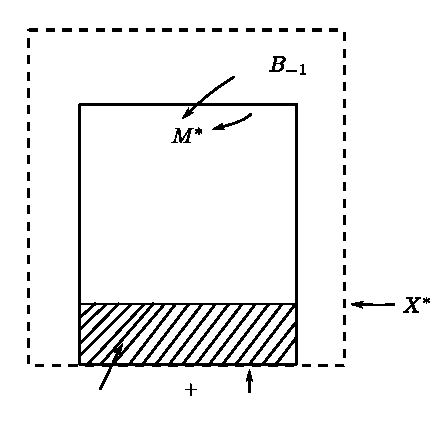
\includegraphics{figure/fig28.eps}
\end{figure}\pageoriginale 

We consider $(M^{*},X^{*})$ as a dual of $(M,X)$. Now $\mathscr{H}$ gives rise to a handle presentation $\mathscr{H}^{*}=(B_{-1},\ldots,B_{n})$ of $(M^{*},X^{*})$ as follows:
\begin{align*}
B_{-1} &= (\p M-X)\times [0,1]\\
B_{k} &= M^{+}-A_{n-k-1}\\
&= B_{k-1}+\mathfrak{h}^{*}_{1}+\cdots+\mathfrak{h}^{*}_{p_{(n-k)}}.
\end{align*}

Where $\mathfrak{h}_{1},\ldots,\mathfrak{h}_{p_{(n-k)}}$ are the $(n-k)$-handles of $\mathscr{H}$. This $\mathscr{H}^{*}$, we will call the dual of $\mathscr{H}$. The number of $k$-handles in $\mathscr{H}$ is equal to the number of $(n-k)$-handles in $\mathscr{H}^{*}$.

Now,
\begin{align*}
& \p M^{*} = X^{*}\cup \overline{\p (A_{-1},X)}\\
\text{so that}\quad & \p (M^{*},X^{*})=\p (A_{-1},X).
\end{align*}

Since $A_{-1}$ is a collar over $\overline{\p(A_{-1},X)}$, this shows that $(M,X)$ is a dual\pageoriginale of $(M^{*},X^{*})$; and with this choice of the dual pair $\mathscr{H}$ is the dual of $\mathscr{H}^{*}$.

Given any handle presentation $\mathscr{K}=(C_{-1},\ldots,C_{n})$ of $(M^{*},X^{*})$ with $C_{-1}=B_{-1}$, then we obviously get a handle presentation $\mathscr{K}^{*}$ of $(M,X)$. Even if $C_{-1}\neq B_{-1}$, we can get a handle presentation of $(M,X)$ whose number of $k$-handles is equal to the number of $(n-k)$-handles of $\mathscr{K}$ as follows:

Let $X^{+}=\overline{\p(M,X)}\times 1$. In $M^{+}$, $C_{-1}\searrow X^{*}$ and $X^{*}\searrow X$, (both) homogeneously. Since $C_{-1}$ is a collar over $X^{*}$; by using the theorems about cells in spheres and cells in cells, we see that $C_{-1}$ is bicollared in $M^{+}$. Moreover $C_{-1}$ is a neighbourhood of $X^{+}$ in $M^{+}$. Hence by the regular neighbourhood theorem, $C_{-1}$ is a regular neighbourhood of $X^{+}$ in $M^{+}$. But $B_{-1}$ is also a regular neighbourhood of $X^{+}$ in $M^{+}$. Therefore, there is an equivalence $f$ of $M^{+}$, fixing $X^{+}$, 
with $f(C_{-1})=B_{-1}$. Since $f(\p M^{+})=\p M^{+}$ and $C_{-1}\cap \p M^{+}=B_{-1}\cap\p M^{+}=X^{*}$, $f$ maps $X^{*}$ onto itself, and as $\p M^{+}=X\cup X^{*}$, $f$ has to map $X$ onto itself. Now the desired handle presentation of $(M,X)$ is given by
\begin{align*}
D_{-1} &= f(A_{-1})\quad(\text{since~ } A_{-1}\searrow X, f(A_{-1})\searrow f(X)=X)\\
D_{k} &= M^{+}-f(C_{n-k-1})\\
&= D_{k-1}+(f(\mathfrak{K}_{1}))^{*}+\cdots +(f(\mathfrak{K}_{p_{(n-k)}}))^{*}
\end{align*}
where $\mathfrak{K}_{1},\ldots,\mathfrak{K}_{p_{(n-k)}}$ are the $(n-k)$-handles of $\mathscr{K}$.

Thus

\subsection{}\label{chap8-sec8.8.1}
If there is a handle presentation of $(M^{*},X^{*})$ without handles of\pageoriginale index $\leq n-\ell$, then there is a handle presentation of $(M,X)$ without handles of index $\geq \ell$. This gives:

\subsection{}\label{chap8-sec8.8.2}
Theorems \ref{chap8-thmA} and \ref{chap8-thmB} imply Theorem \ref{chap8-thmC}.

Since $X\hookrightarrow M$ is a homotopy equivalence and $\pi_{1}(M)\approx \pi_{1}(\p(M,X))$, using duality in the universal covering spaces, that is $H_{i}(M^{*},X^{*})\approx H^{n-i}(M,X)=0$, we see that $X^{*}\hookrightarrow M^{*}$ is also a homotopy equivalence. If $n\geq 6$, then we can find a handle presentation of $(M^{*},X^{*})$ without handles of index $\leq 6-4=2$ by Theorem \ref{chap8-thmA}. Hence we can obtain handle presentation $\mathscr{H}$ of $(M,X)$ without handles of index $\geq n-2$, that is, with handles of index $\leq n-3$ only. But then, by Theorem \ref{chap8-thmB}, as $\tau(M,X)=0$, we can get from $\mathscr{H}$ a handle presentation of $(M,X)$ without any handles, that is $M\searrow X$.

\subsection{}\label{chap8-sec8.8.3}
If $n=5$, and $(M,X)$ is a $h$-cobordism, then there is a handle presentation of $(M,X)$ with only $2$- and $3$-handles.

\setcounter{proposition}{3}
\begin{ex}
A (compact) contractible PL $2$-manifold is a $2$-cell.
\end{ex}

\section{Algebraic Description}\label{chap8-sec8.9}

We have already remarked (\ref{chap8-sec8.3.7}) that there is a certain algebraic structure associated to a handle presentation $\mathscr{H}=(A_{-1},\ldots,A_{n})$ of a relative $n$-manifold $(M,X)$. We suppose now that $(M,X)$ is a special case, and that there are no $0$- or $1$-handles in $\mathscr{H}(A_{-1}=A_{0}=A_{1})$. Also $n\geq 3$ and $\pi_{1}(X)\to \pi_{1}(M)$ is an isomorphism. This we will call Hypothesis 

\subsection{}\label{chap8-sec8.9.1}
 In this case, the maps
\begin{equation*}
\pi_{1}(X)\to \pi_{1}(A_{-1})\to \ldots\to \pi_{1}(A_{n})  
\end{equation*}
are all isomorphisms. The reason $\pi_{1}(A_{1})\to \pi_{1}(A_{2})$ is an isomorphism is\pageoriginale that $\pi_{1}(X)\to \pi_{1}(M)$ is an isomorphism and $\pi_{1}(A_{1})\to \pi_{1}(A_{2})$ is a surjection. We identity all these groups and call it $\pi$.

Now, the groups
$$
C_{i}=\pi_{i}(A_{i},A_{i-1})
$$
are identified with $H_{i}(\tilde{A}_{i},\tilde{A}_{i-1})$. They are free modules over $Z\pi$ with bases corresponding to handles. $\mathscr{H}\{\mathfrak{h}^{(i)}_{1},\ldots,\mathfrak{h}^{(i)}_{p_{i}}\}$ are the $i$-handles, the basis of $C_{i}$ is denoted by $\{[\mathfrak{h}^{(i)}_{1}],\ldots,[\mathfrak{h}^{(i)}_{p_{i}}]\}$ and the elements of this basis are well defined upto multiplying by elements $\pm \pi$.

If $f:A_{k}\to A_{k}$ is a polyhedral equivalence isotopic to the identity, it is easily seen that the algebraic structures already described for $\mathscr{H}$ and $\mathscr{H}_{f}$ may be identified.

In addition, we have a map
$$
\p_{k}:C_{k}\to C_{k-1}
$$
which is the boundary map of the triple $(A_{k},A_{k-1},A_{k-2})$. This is also unchanged by changing $\mathscr{H}$ to $\mathscr{H}_{f}$.

If there are no handles of index $\leq k-2$ and $\pi_{k-1}(M,X)=0$, we see:

First, $\pi_{k-1}(A_{k},A_{k-2})=0$, and hence from the exact sequence of the triple $(A_{k},A_{k-1},A_{k-2})$ the map $\p_{k}:C_{k}\to C_{k-1}$ is surjective.

Dually, if there are no handles of index $>k$ and $\pi_{k}(X,X)=0$, we have 
$$
\p_{k}:C_{k}\to C_{k-1}\quad\text{ to be injective.}
$$\pageoriginale

Now, the boundary map $\p_{k}$ plus the bases of $C_{k}$ and $C_{k-1}$ determine a matrix $B_{k}$ in the usual way. That is, if
$$
\p_{k}\left([\mathfrak{h}^{(k)}_{i}]\right)=\sum^{p_{(k-1)}}_{j=1}\alpha_{i,j}[\mathfrak{h}^{(k-1)}_{j}],\alpha_{i,j}\in Z\pi
$$
then $B_{k}$ is the $p_{k}\times p_{(k-1)}$ matrix
$$
\begin{bmatrix}
\alpha_{1,1} & \alpha_{1,2} & \ldots & \alpha_{1,p_{(k-1)}}\\
\alpha_{2,1} & \alpha_{2,2} & \ldots & \alpha_{2,p_{(k-1)}}\\
\vdots & \vdots & \vdots & \vdots\\
\alpha_{p_{k},1}, & \alpha_{p_{k},2} & \ldots & \alpha_{p_{k},p_{k-1}}
\end{bmatrix}
$$

If we choose a different orientation of core of $\mathfrak{h}_{i}^{(k)}$, then $[\mathfrak{h}^{(k)}_{i}]$ is replaced by - $[\mathfrak{h}^{(k)}_{i}]$ (in the basis of $C_{k}$) so that the $i^{\text{th}}$ row of $B_{k}$ is multiplied by $-1$. If we extend the handle $\mathfrak{h}^{(k)}_{i}$ along a path representing $\alpha\in \pi$, then $[\mathfrak{h}^{(k)}_{i}]$ is replaced by $\alpha[\mathfrak{h}^{(k)}_{i}]$, so that the $i^{\text{th}}$ row of $B_{k}$ is multiplied by $\alpha$. Thus, by different choices of orientations of cores and paths to the ``base point'', we  can change $B_{k}$ somewhat. There is another type of modification which we can do on $B_{k}$: that is adding a row of $B_{k}$ to another row of $B_{k}$. This is done by using \ref{chap8-sec8.6.3} as follows:

Consider two $k$-handles $\mathfrak{h}^{(k)}_{i}$ and $\mathfrak{h}^{(k)}_{j}$ of $\mathscr{H}$, and let\pageoriginale $2\leq k\leq n-2$. We now apply \ref{chap8-sec8.6.3} (Remark 2), with $A_{k-1}=N$, $\overline{\p (A_{k-1},X)}=N'$, $\mathfrak{h}^{(k)}_{i}=\mathfrak{h}_{1}$, $\mathfrak{h}^{(k)}_{j}=\mathfrak{h}_{2}$. This gives a new handle $\mathfrak{h}^{(k)}$, away from $\mathfrak{h}^{(k)}_{i}$ and $\mathfrak{h}^{(k)}_{j}$, such that
$$
A_{k-1}+\mathfrak{h}^{(k)}+\mathfrak{h}^{(k)}_{j}\approx A_{k-1}+\mathfrak{h}^{(k)}_{i}+\mathfrak{h}^{(k)}_{j}
$$
and $\p[\mathfrak{h}]$, with proper choices, now represents $[\mathfrak{h}^{(k)}_{i}]\pm\theta[\mathfrak{h}^{(k)}_{j}]$, (sign prescribed), in $\pi_{k-1}(\p (A_{k-1},X))$. Also, we can assume that $\mathfrak{h}^{(k)}$ is away from the attaching tubes of the other handles, so that 
\begin{gather*}
B=(A_{k-1}+\mathfrak{h}^{(k)})+\mathfrak{h}^{(k)}_{j}\quad(\text{other~ }p_{k}^{-2} k\text{-handles of~ } \mathscr{H})\\
{\displaystyle{\mathop{\approx}^{\psi}}}A_{k},
\end{gather*}
and $\psi$ can be assumed to be identity on $X$.

Now $(B,X)$ has an obvious handle presentation $\mathscr{K}=(B_{-1},\ldots,B_{n})$, where
\begin{align*}
& B_{i}=A_{i,i\leq k-1}\\
& B_{k}=B.
\end{align*}

The $k^{\text{th}}$ boundary map of $\mathscr{K}$, with the appropriate bases, has a matrix which is the same as $B_{k}$ except for $i^{\text{th}}$ row, which is now replaced by the sum of the $i^{\text{th}}$ row + $(\pm \theta)$ times the $j^{\text{th}}$ row, corresponding to the relation
$$
\p[\mathfrak{h}^{(k)}]=\p[\mathfrak{h}_{i}^{(k)}]\pm \theta \p [\mathfrak{h}^{(k)}_{j}]
$$

We pull $\mathscr{K}$ to a handle presentation $\mathscr{K}'$ of $(A_{k},X)$ by $\psi$. In $\mathscr{K}$ and $\mathscr{K}'$, the matrices of the boundary maps are the same if we choose the\pageoriginale corresponding bases. And $\mathscr{K}'$ can be extended to handle presentation $\mathscr{H}'$ of $(M,X)$ by adding the $(\geq k+1)$-handles as they are. By doing a finite number of such changes, we have

\subsection{(Basis Lemma).}\label{chap8-sec8.9.2}
$\mathscr{H}$ is a handle presentation satisfying \ref{chap8-sec8.9.1}, $B_{k}$ is the matrix of the $k^{\text{th}}$ boundary of map of $\mathscr{H}_{1}^{(k\leq n-2)}$, with respect to bases corresponding to handles. Given any $p_{k}\times p_{k}$ matrix $E$ which is the product of elementary matrices, then $\exists$ a handle presentation $\mathscr{H}'$ of $(M,X)$ satisfying \ref{chap8-sec8.9.1}
\begin{itemize}
\item[(1)] the number of $i$-handles in $\mathscr{H}$ is the same as the number of $i$-handles in $\mathscr{H}'$, for all $i$, and

\item[(2)] the matrix of the $k^{\text{th}}$ boundary map of $\mathscr{H}'$ with appropriate bases corresponding to handles is $E\cdot B_{k}$.
\end{itemize}

As an application of the ``Basis Lemma'', we will prove a proposition, usually known as the ``Existence Theorem for $h$-cobordisms''. Let $M$ be a PL $(n-1)$-manifold; $M$ compact, with or without boundary. The problem is to produce a PL $n$-manifold $W$ containing $M$ in its boundary such that $(W,M)$ is a $h$-cobordism with prescribed torsion.

\setcounter{proposition}{2}
\begin{proposition}\label{chap8-prop8.9.3}
If the dimension of $M$ is greater than $4$, then given any $\tau_{0}\in Wh(\pi_{1},(M))$, there exists a $h$-cobordism $(W,M)$ with $\tau(W,M)=\tau_{0}$.
\end{proposition}

\begin{proof}
Let $A=(a_{ij})$ be a matrix $(m\times m)$ representing $\tau_{0}$. Consider $N=M\times I$, identify $M$ with $M\times 0$. To $(N,M)$ attach $m$ cancelling pairs of $2$- and $3$-handles and $m$ $3$-handles away from these. Let $W'$ be the resulting manifold: and let $\mathscr{H}$ be the obvious handle\pageoriginale 
presentation of $(W',M)$; $\mathscr{H}$ satisfies \ref{chap8-sec8.9.1}. Then the matrix of the $3^{\text{rd}}$ boundary map of $\mathscr{H}$ with appropriate bases is $\left[\begin{smallmatrix} I_{m}\\ 0_{m}\end{smallmatrix}\right]$. Consider the matrix $\left[\begin{smallmatrix} A & 0\\ 0 & A^{-1}\end{smallmatrix}\right]$; this is a product of elementary matrices. Hence by \ref{chap8-sec8.9.2}, we can obtain a new handle presentation $\mathscr{H}'$ of $(W',M)$ satisfying \ref{chap8-sec8.9.1}, such that the number of handles of each index is the same in $\mathscr{H}$ and $\mathscr{H}'$, and the $3^{\text{rd}}$ boundary map of $\mathscr{H}'$ with bases corresponding to handles is 
$$ 
\begin{bmatrix}
A & 0\\ 
0 & A^{-1} 
\end{bmatrix}
\begin{bmatrix}
I_{m}\\
0_{m}
\end{bmatrix}
=
\begin{bmatrix}
A \\ 0_{m}
\end{bmatrix}
$$

Thus, if $\mathfrak{K}_{1},\ldots,\mathfrak{K}_{2m}$ are the 3-handels and $\mathfrak{h}_{1},\ldots,\mathfrak{h}_{m}$ the $2$-handles of $\mathscr{H}'$, and $[\mathfrak{K}_{i}]$, $[\mathfrak{h}_{i}]$ denote the corresponding basis elements, then
\begin{align*}
& \p[\mathfrak{K}_{i}]=\sum^{m}_{j=1}a_{ij}[\mathfrak{h}_{j}],\quad \text{if}\quad i\leq m\\
& \p[\mathfrak{K}_{i}]=0\qquad \text{if}\quad i>m.
\end{align*}

Let $W$ be the manifold $W'-(\mathfrak{K}_{m+1}\cup\ldots\cup \mathfrak{K}_{2m})$. Let $\mathscr{K}$ be the handle presentation of $(W,N)$ given by $\mathfrak{h}_{i}$'s and $\mathfrak{K}_{i}$'s for $i\leq m$. Then the $3^{\text{rd}}$ boundary map of $\mathscr{K}$ has the matrix $A$. Clearly $M\hookrightarrow W$ is a homotopy equivalence ($A$ is non-singular). Since, dually we are attaching $n-2$ and $n-3$ handles to $\overline{\p (W,M)}$ to get $W$, and $n-3\geq 3$, $\pi_{1}(\p (W,M))\to \pi_{1}(W)$ is an isomorphism. Hence $(W,M)$ is a $h$-cobordism with the prescribed torsion $\tau_{0}$.
\end{proof}

Again,\pageoriginale consider a handle presentation $\mathscr{H}$ satisfying \ref{chap8-sec8.9.1}. For $k\leq n-3$, $A_{k}$ is, upto homotopy obtained by attaching cells of dimension $\geq 3$ to $\p(A_{k},X)$. This shows, $\pi_{1}(\p(A_{k},X))\to \pi_{1}(A_{k})$ is an isomorphism for $k\leq n-3$; and hence $\widetilde{\p(A_{k},X)}=\p(\tilde{A}_{k},\tilde{X})$. 

We are interested in the following question:

Suppose a $k$-sphere $\sum\subset (A_{k},X)$ represents in $\pi_{k}(A_{k},A_{k-1})$ the element $[\mathfrak{h}]$ corresponding to a particular $k$-handle. Then, is there a map $f:\sum\to \p(A_{k},X)$ homotopic to the inclusion of $\sum$ in $\p(A_{k},X)$, such that $f|a$ hemisphere of $\sum$ is an embedding onto a core of $\mathfrak{h}$?

We note that $\p(A_{k},X)\cap \p(A_{k-1},X)$
\begin{quote}
$=\p(A_{k},X)$ - (transverse tubes of $k$-handles)

$=\p(A_{k-1},X)$ - (attaching tubes of $k$-handles)
\end{quote}
and so $\p(A_{k},X)\cap \p(A_{k-1},X)$ will have fundamental group $\pi$ if either $(n-k-1)\leq (n-1)-3$ or $(k-1)\leq (n-1)-3$, so that $k\leq (n-3)$ is sufficient. This implies
\begin{align*}
\widetilde{\p(A_{k},X)\cap \p(A_{k-1},X)} &= \widetilde{\p(A_{k},X)}\cap \p\widetilde{(A_{k-1},X)}\\
&= \p(\tilde{A}_{k},\tilde{X})\cap\p(\tilde{A}_{k-1},\tilde{X}).
\end{align*}

Consider\pageoriginale the following diagram:
\[
\xymatrix{
\pi_{k}(\p (A_{k},X),\p(A_{k},X)\cap \p(A_{k-1},X))\ar[r]^-{i_{1}} & \pi_{k}(A_{k},A_{k-1})\\
\pi_{k}(\p(\tilde{A}_{k},\tilde{X}),\p(\tilde{A}_{k},\tilde{X})\cap \p(\tilde{A}_{k-1},\tilde{X}))\ar[u]_{\alpha_{1}}\ar[r]^-{i_{2}}\ar[d]^{\mathfrak{h}_{1}} & \pi_{k}(\tilde{A}_{k},\tilde{A}_{k-1})\ar[d]^{\mathfrak{h}_{2}}\ar[u]_{\alpha_{2}}\\
H_{k}(\p(\tilde{A}_{k},\tilde{X}),\p(\tilde{A}_{k},\tilde{X})\cap \p(\tilde{A}_{k-1},\tilde{X}))\ar[r]^-{i_{3}} & H_{k}(\tilde{A}_{k},\tilde{A}_{k-1}).
}
\]

Here $h_{1}$, $h_{2}$ are hurewicz maps, $i_{1}$, $i_{2}$, $i_{3}$ are induced by inclusion maps, $\alpha_{1}$ and $\alpha_{2}$ are the maps induces by $\tilde{M}\to M$. All the induces occuring are $\geq 2$. $\alpha_{1}$ and $\alpha_{2}$ are well known to be isomorphims. $h_{1}$ and $h_{2}$ are isomorphisms since the pairs are $(k-1)$-connected. By excision, $i_{3}$ is an isomorphism. Hence $i_{2}$ and $i_{1}$ are also isomorphisms. Therefore, a boundary core of $\mathfrak{h}$ and $\sum$ represent the same element in $\pi_{k}(\p(A_{k},X),\p(A_{k},X)\cap \p(A_{k-1},X))$.

Thus the answer to out question is Yes:

\setcounter{subsection}{3}
\subsection{}\label{chap8-sec8.9.4}
Let $\mathscr{H}$ be a handle presentation satisfying the hypothesis \ref{chap8-sec8.9.1}. Let $k$ be an integer $\leq n-3$ [or $k\geq 3$, $\pi_{1}(\p(A_{k},X))\to \pi_{1}(A_{k})$ is an isomorphism, $k\leq n-1$]. Then two geometric objects, representing the same element of $\pi_{k}(A_{k},A_{k-1})$, also represent the same element of $\pi_{k}(\p(A_{k},X), \p(A_{k},X)\cap \p(A_{k-1},X))$. In particular, if $\sum\subset \p(A_{k},X)$ is a $k$-sphere, representing the element $[\mathfrak{h}]$ in $\pi_{k}(A_{k},A_{k-1})$; then it\pageoriginale represents the element $[\mathfrak{h}]$ in $\pi_{k}(\p(A_{k},X),\p(A_{k},X)\cap \p(A_{k-1},X))$. This means that there is a homotopy in $\p(A_{k},X)$ from the identity map of $\sum$ of a map taking the upper hemisphere of $\sum$ in a $1-1$ way onto a (boudnary) core of $\mathfrak{h}$, and taking the lower hemisphere of into $\p(A_{k},X)\cap \p(A_{k-1},X)$; in particular the end result of $\sum$ will not intersect any other handles.

If $\sum$ is the attaching sphere of a $(k+1)$-handle $\mathfrak{K}$ and $\p_{k+1}([\mathfrak{K}])=[\mathfrak{h}]$, we have the above situation. We would like to get a suitable isotopy from the above homotopy information, to cancel the handles corresponding $\mathfrak{K}$ and $\mathfrak{h}$ in some $\mathscr{H}_{f}$. This is provided by the following lemma. Since the proof of this lemma is rather long and seems to be of some general interest, we will postpone the proof to the last section.

\subsection{(Isotopy Lemma).}\label{chap8-sec8.9.5}
With the hypotheses of \ref{chap8-sec8.9.4}, if $n$ addition, $n\geq 6$ and $k\leq n-4$, then there is an isotopy in $\p(A_{k},X)$ carrying $\sum$ to another $k$-sphere $\sum'$, such that $\sum'$ intersects a transverse sphere of $\mathfrak{h}$ in one point transversally and does not intersect the other $k$-handles.

\section{Proofs of Theorems \ref{chap8-thmA} and \ref{chap8-thmB}}\label{chap8-sec8.10}

In this section, we will prove Theorems \ref{chap8-thmA} and \ref{chap8-thmB} assuming the Isotopy Lemma, which will be proved in the next section.

First let us see what are the types of manifolds and presentations that we have to consider. Theorem \ref{chap8-thmA}, for $\ell\leq 1$ is proved in \ref{chap8-sec8.7}. So, we can assume $\ell\geq 2$, and hence $n\geq 6$. For Theorem \ref{chap8-thmB}, $\ell=n$ and $n\geq 6$, by hypothesis. So again using \ref{chap8-sec8.7}, it is enough to consider handle\pageoriginale presentations satisfying \ref{chap8-sec8.9.1}, and in addition $n\geq 6$.

We start with two observations concerning the matrices of the\break boundary maps:

\subsection{}\label{chap8-sec8.10.1}
Let $\mathscr{H}$ be handle presentation satisfying \ref{chap8-sec8.9.1}, $\mathfrak{h}^{(i)}_{1},\ldots,\mathfrak{h}^{(i)}_{p_{i}}$ be the $i$-handles of $\mathscr{H}$. Let $B_{k+1}=(\alpha_{ij})$ be the matrix of the $(k+1)^{\text{st}}$ boundary map $\p_{k+1}$ with respect to preferred bases. That is, 
$$
\p_{k+1}\left(\left[\mathfrak{h}^{(k+1)}_{i}\right]\right)=\sum^{p_{k}}_{j=1}\alpha_{ij}[\mathfrak{h}^{(k)}_{j}],\quad\alpha_{ij}\in Z(\pi).
$$

Suppose $\mathfrak{h}^{(k)}_{1}$ and $\mathfrak{h}^{(k+1)}_{1}$ can be cancelled. Then we have formed a handle presentation $\mathscr{H}-(\mathfrak{h}^{(k)}_{1},\mathfrak{h}^{(k+1)}_{1})=(B_{-1},\ldots,B_{n})$ say, of $(M,X)$ as follows:
\begin{align*}
& B_{i}=f(A_{i})\quad\text{for}\quad i<k\\
& B_{k}=f(A_{k}-\mathfrak{h}^{(k)}_{1})=A_{k}+\mathfrak{h}_{1}^{(k+1)}\\
& B_{i}=A_{i}\quad\text{for}\quad i>k.
\end{align*}

Here $f$ is an equivalence $A_{k}-\mathfrak{h}^{(k)}_{1}\approx A_{k}+\mathfrak{h}^{(k+1)}_{1}$ mapping $X$ onto itself. If the attaching tube of $\mathfrak{h}^{(k+1)}_{1}$ does not intersect any other $k$-handle except $\mathfrak{h}^{(k)}_{1}$, $f$ can be assumed to be identity on all $\mathfrak{h}^{(k)}_{i}$, $i\geq 2$. We assume that this is the case. Now $\mathfrak{h}^{(k)}_{2},\ldots,\mathfrak{h}^{(k)}_{p_{k}}$ are all the $k$-handles and $\mathfrak{h}^{(k+1)}_{2},\ldots,\mathfrak{h}^{(k+1)}_{p_{(k+1)}}$ are all the $(k+1)$-handles of $\mathscr{H}-(\mathfrak{h}^{(k)}_{1},\mathfrak{h}^{(k+1)}_{1})$. Thus (by abuse of notation) $[\mathfrak{h}^{(k)}_{2}],\ldots,[\mathfrak{h}^{(k)}_{p_{k}}]$ is a basis of $\pi_{k}(B_{k},B_{k-1})$ and\pageoriginale $[\mathfrak{h}^{(k+1)}_{2}],\ldots,[\mathfrak{h}^{(k+1)}_{p_{(k+1)}}]$ is a basis of $\pi_{k+1}(B_{k+1},B_{k})$. Let $\partial'_{k+1}$ denote the $(k+1)^{\text{st}}$ boundary map of $\mathscr{H}-(\mathfrak{h}^{(k)}_{1},\mathfrak{h}^{(k+1)}_{1})$. Consider the following commutative diagram $(A_{k+1}=B_{k+1},A_{k}\subset B_{k},A_{k-1}\subset B_{k-1})$: 
\[
\xymatrix{
\pi_{k+1}(A_{k+1},A_{k})\ar[d]^{i_{1_{\ast}}}\ar[r]^-{\p} & \pi_{k}(A_{k})\ar[d]^{i_{2_{\ast}}}\ar[r]^-{j} & \pi_{k}(A_{k},A_{k-1})\ar[d]^{i_{3_{\ast}}}\\
\pi_{k+1}(B_{k+1},B_{k})\ar[r]^{\p'} & \pi_{k}(B_{k})\ar[r]^{j'} & \pi_{k}(B_{k},B_{k-1})
}
\]

In this diagram, the vertical maps are induced by inclusion, the horizontal maps are canonical maps, and $j\circ \p =\p_{k+1}$, $j'\circ\p'=\p'_{k+1}$. Now
\begin{align*}
& i_{1_{\ast}}\left([\mathfrak{h}^{(k+1)}_{1}]\right)=0\\
& i_{1_{\ast}}\left([\mathfrak{h}^{(k+1)}_{i}]\right)=[\mathfrak{h}_{i}^{(k+1)}]\quad\text{for}\quad i\geq 2.
\end{align*}
and 
\begin{align*}
& i_{3_{0}}\left([\mathfrak{h}^{(k)}_{1}]\right)=0,\\
& i_{3_{\ast}}\left([\mathfrak{h}^{(k)}_{i}]\right)=\left([\mathfrak{h}^{(k)}_{i}]\right)\quad\text{for}\quad i\geq 2.
\end{align*}

Hence, for $i\geq 2$,
\begin{align*}
& \p'_{k+1}\left([\mathfrak{h}^{(k+1)}_{i}]\right)\\
&=\p'_{k+1}\circ i_{1_{\ast}}\left([\mathfrak{h}^{(k+1)}_{i}]\right)\\
&=j'\circ \p'\circ i_{1_{\ast}}\left([\mathfrak{h}^{(k+1)}_{i}]\right)\\
&=i_{3_{\ast}}\circ j\circ \p\left([\mathfrak{h}^{(k+1)}_{i}]\right)\\
&= i_{3_{\ast}}\circ \p_{k+1}\left([\mathfrak{h}^{(k+1)}_{i}]\right)\\
&= i_{3_{\ast}}\left(\sum^{p_{k}}_{i=1}\alpha_{ij}[\mathfrak{h}^{(k)}_{j}]\right)\\
&= \sum^{p_{k}}_{i=2}\alpha_{ij}\left([\mathfrak{h}^{(k)}_{j}]\right)
\end{align*}\pageoriginale 

Thus, if the matrix of $\p_{k+1}$ is $(\alpha_{ij})$, then the matrix of $\p'_{k+1}$ is $(\alpha_{ij})$, $i\geq 2$, $j\geq 2$. This we have as long as the attaching tube of $\mathfrak{h}^{(k+1)}_{1}$ keeps away from the transverse tubes of the handles $\mathfrak{h}^{(k)}_{i}$, $i\geq 2$. (It is easy to see that $\alpha_{1,2}=\ldots=\alpha_{1,pk}=0$, in this case). It does not matter even if the attaching tubes of other $(k+1)$-handles intersect the transverse tube of $\mathfrak{h}^{(k)}_{1}$.

\subsection{}\label{chap8-sec8.10.2}
If $f:A_{k}\to A_{k}$ is an equivalence isotopic to the identity leaving $X$ fixed, then in $\mathscr{H}^{f}$ and $\mathscr{H}$, the attaching spheres of the corresponding $(k+1)$-handles represent the same elements in $\pi_{k}(A_{k})$. Since the $(k+1)^{\text{st}}$ boundary maps are factored through $\pi_{k}(A_{k})$, the corresponding matrices are the same after the choice of obvious bases in $\mathscr{H}$ and $\mathscr{H}^{f}$, and hence in $\mathscr{H}$ and $\mathscr{H}(f^{-1})$. 

\medskip
\noindent
{\bf Proof of Theorem A.}
\setcounter{step}{0}
\begin{step}%1
Let $\mathscr{H}=(A_{-1},\ldots,A_{n})$ be a handle presentation of $(M,X)$ satisfying \ref{chap8-sec8.9.1}. We are given that $(M,X)$ is $\ell$-connected, then we know that the sequence
\begin{equation*}
\pi_{\ell+1}(A_{\ell+1},A_{\ell})\to \pi_{\ell}(A_{\ell},A_{\ell-1})\to\ldots \pi_{2}(A_{2},A_{-1})\to 0
\end{equation*}\pageoriginale
is exact.
\end{step}

Suppose that we have already eliminated upto handles of index $(i-1)$, that is in $\mathscr{H}$, $A_{-1}=A_{0}=\ldots=A_{i-1}$; then by (*), $\pi_{i+1}(A_{i+1},A_{i})\xrightarrow{\p_{i+1}}\pi_{i}(A_{i},A_{i-1})$ is onto. Let $B_{i+1}$ be the matrix $(p_{i+1}\times p_{i})$ of $\pi_{i+1}$ with bases corresponding to handles. Then, there exists a $(p_{i+1}+p_{i})\times(p_{i+1}+p_{i})$ matrix $E$, which is the product of elementary matrices, such that
\begin{equation*}
E\times 
\begin{bmatrix}
B_{i+1}\\
0_{p_{i}}
\end{bmatrix}
=
\begin{bmatrix}
I_{p_{i}}\\
0_{p_{i+1},p_{i}}
\end{bmatrix}.
\end{equation*}

If we attach $p_{i}$ cancelling pairs of $(i+1)$, $(i+2)$-handles away from the handles of index $\leq (i+2)$ to the $i^{\text{th}}$ level of $\mathscr{H}$, then in the resulting handle presentation $(B_{-1},\ldots,B_{n})$ of $(M,X)$, the matrix of $\pi_{i+1}(B_{i+1},B_{i})\to \pi_{k}(B_{i},B_{i-1})$ with appropriate bases is$$
\begin{bmatrix}
B_{i+1}\\
0_{p_{i}}
\end{bmatrix}.
$$

Then, by the Basis Lemma, we can obtain a handle presentation of $(M,X)$ satisfying \ref{chap8-sec8.9.1}, with exactly the same number of handles of each index as above, but $(i+1)^{\text{st}}$ boundary matrix will now be 
$$
E\times
\begin{bmatrix}
B_{i+1}\\
0_{p_{i}}
\end{bmatrix}
=
\begin{bmatrix}
I_{p_{i}}\\
0_{p_{i+1},p_{i}}
\end{bmatrix}
$$\pageoriginale

This means that starting from $\mathscr{H}$, we can obtain a handle presentation $\mathscr{K}=(C_{-1},\ldots,C_{n})$ of $(M,X)$ such that 
\begin{enumerate}
\renewcommand{\labelenumi}{(\theenumi)}
\item $\mathscr{K}$ satisfies \ref{chap8-sec8.9.1}, and there are no handles of indices $\leq i-1$

\item the $(i+1)^{\text{st}}$ boundary map of $\mathscr{K}$ has the matrix $\left[\begin{smallmatrix} I_{p_{i}}\\ 0\end{smallmatrix}\right]$.
\end{enumerate}

Now we can eliminate the $i$-handles one at a time as follows:

\begin{step}%2
Consider $\mathfrak{h}^{(i+1)}_{1}$ and $\mathfrak{h}^{(i)}_{1}\cdot \p_{i+1}([\mathfrak{h}^{(i+1)}_{1}])=[\mathfrak{h}^{(i)}_{1}]$; and $i\leq n-4$. Hence by the Isotopy Lemma, there is an equivalence $f$ of $\p(C_{i},X)$, such that $f$ takes an attaching sphere $S_{1}$ of $\mathfrak{h}_{1}^{(i+1)}$ to another $i$-sphere $S'_{1}$ and $S'_{1}$ intersects a transverse sphere of $\mathfrak{h}^{(i)}_{1}$ at one point transversally. Moreover it can be assumed that $f$ (attaching tube of $\mathfrak{h}^{(i+1)}_{1}$) does not intersect the transverse tubes of the other          $i$-handles. $f$ can be extended to an equivalence $f$ of $C_{i}$ taking $X$ onto itself and in $\mathfrak{K}^{f}$ the handles corresponding $\mathfrak{h}^{(i)}_{1}$ and $\mathfrak{h}^{(i+1)}_{1}$ can be nearly cancelled. By \ref{chap8-prop8.5.7}, there is an equivalence $g$ of $C_{i}$, so that in $(\mathscr{K}^{f})^{g}=\mathscr{K}^{(gf)}$, the handles corresponding $\mathfrak{h}^{(i)}_{1}$ and $\mathfrak{h}^{(i+1)}_{1}$ can be cancelled. Again, we can require that $g\circ f$ (attaching tube of $\mathfrak{h}^{(i+1)}_{1}$) should not intersect the transverse tubes of handles $\mathfrak{h}^{(i)}_{j}$, $j\geq 2$. Consider $\mathscr{K}_{{(gf)^{-1}}}$. This is a handle-presentation\pageoriginale of $(M,X)$, and in $\mathscr{K}_{(gf)^{-1}}$ the handles $\mathfrak{K}^{(i)}_{1}$ and $\mathfrak{K}^{(i+1)}_{1}$ say, corresponding to $\mathfrak{h}^{(i)}_{1}$ and $\mathfrak{h}^{(i+1)}_{1}$ can be cancelled. By \ref{chap8-sec8.10.1}, and since $f$ and $g$ can be assumed to be isotopic to identity, the $(i+1)^{\text{st}}$ boundary map of $\mathscr{K}_{(gf)^{-1}}-(\mathfrak{K}^{(i)}_{1},\mathfrak{K}^{(i+1)}_{1})$ has the matrix $\left[\begin{smallmatrix}I_{(p_{i}-1)}\\ 0\end{smallmatrix}\right]$. Hence, we can go on repeating step 2 to obtain a handle presentation of $(M,X)$ without handles upto index $i$.

Thus, inductively, the first part of Theorem A is proved. The second part is clear.
\end{step}


\noindent
{\bf Proof of Theorem B:} By Theorem A, we can assume that there is a handle presentation $\mathscr{H}$ of $(M,X)$ with handles of indices $(n-3)$ and $(n-4)$ only. $\mathscr{H}$ obviously satisfies \ref{chap8-sec8.9.1}. Consider the map
$$
\p_{n-3}:\pi_{n-3}(A_{n-3},A_{n-4})\to \pi_{n-4}(A_{n-4},A_{n-5}).
$$

Here $A_{-1}=\ldots=A_{n-5}$. Let $A$ be the matrix of $\p_{n-3}$ with respect to bases corresponding to handles. $A$ is a nonsingular matrix, say $m\times m$ matrix. Since $\tau(M,X)=0$, $A$ represents the $0$-element in $Wh(\pi)$. Hence for some $q\leq m$ there exists an $(m+q)\times (m+q)$ matrix $E$ which is the product of elementary matrices, such that 
$$
E\times 
\begin{bmatrix}
A &0\\
0 & I_{q}
\end{bmatrix}
=I_{m+q}
$$

Now we add $q$ cancelling pairs of $(n-3)$- and $(n-4)$-handles to $A_{n-5}$ away from the other handles, so that in the new handle presentation, say $\mathscr{K}$, of $(M,X)$, the $(n-3)^{\text{rd}}$ boundary map of $\mathscr{K}$ has the matrix
$$
\begin{bmatrix}
A &0\\
0 & I_{q}
\end{bmatrix}.
$$

Then\pageoriginale by the Basis Lemma, we can obtain a new handle presentation $\mathscr{K}'$ of $(M,X)$ with exactly $(m+q)$ handles of indices $(n-3)$ and $(n-4)$ and no others, and such that the matrix of the $(n-3)^{\text{rd}}$ boundary map of $\mathscr{K}'$ with respect to bases corresponding to handles is $I_{m+q}$. Now, by a repeated application of Step 2 in the proof the Theorem A, all the handles can be eliminated so that $M\searrow X$.

\section{Proof of the Isotopy Lemma}\label{chap8-sec8.11}

We begin with some elementary lemmas.

\begin{lemma}\label{chap8-lem8.11.1}
Let $Q\subset P$, $Y\times \Delta \subset X$ be polyhedra, where $\Delta$ is $k$-cell and $\dim Q\leq k$ and $f:p\to X$ a polyhedral map. Then the set of points $\alpha\in\Delta$ such that $Q\cap f^{-1}(Y\times\alpha)=\emptyset$ contains an open and dense subset of $\Delta$.
\end{lemma}

\begin{proof}
Let $Q'=f(Q)\cap (Y\times \Delta)$. Then $\dim Q'\leq \dim Q<k$. The projection of $Q'$ to $\Delta$ does not cover most of the points of $k$-dimensional $\Delta$. Any point $\alpha$ not belonging to the projection of $Q'$ to $\Delta$ will satisfy $Q\cap f^{-1}(Y\times \alpha)=\emptyset$.
\end{proof}

\begin{lemma}\label{chap8-lem8.11.2}
If $\dim Q=k$ in the above, then the set of points $\alpha\in\Delta$ such that $Q\cap f^{-1}(Y\times \alpha)$ is $0$-dimensional contains an open and dense subset of $\Delta$.
\end{lemma}

\begin{proof}
Triangulate the projection of $Q'$ to $\Delta$. If $\mathscr{A}$ is the simplicial presentation of $\Delta$ with respect to which this map is simplicial, then every point $\alpha$ of $\Delta-|\mathscr{A}_{k-1}|$ will have the above property by \ref{chap4-sec4.2}.
\end{proof}

Let $f:P\to X$ be a nondegenerate map, simplicial with respect to the presentations $\mathscr{P}$, $\mathscr{X}$ of $P$, $X$. Let $\sum(f)$ denote the closure of the set $S(f)=\{x\in P|\exists y\in P, y\neq x,f(y)=f(x)\}$ (see \ref{chap5-sec5.4}).\pageoriginale $\sum(f)$ is covered by a subpresentation of $\mathscr{P}$, call it $\sum$. 

\setcounter{subsection}{2}
\subsection{}\label{chap8-sec8.11.3}
If $\sigma$ is a principal simplex of $\sum$, then $f||St(\sigma,\mathscr{P})|$ is an embedding.

\begin{proof}
Since $f$ is nondegenerate it maps $Lk(\sigma,\mathscr{P})$ into $Lk(f\sigma,\mathscr{X})$ and on $|St(\sigma,\mathscr{P})|$ it is the join of $\overline{\sigma}\to \overline{f\sigma}$ and $|Lk(\sigma,\mathscr{P}|\to |Lk(f\sigma,\mathscr{X})|$. The map $|Lk(\sigma,\mathscr{P})|\to |Lk(f\sigma,\mathscr{X})|$ is an embedding; otherwise if $\tau_{1}\neq \tau_{2}$, $\tau_{1}$, $\tau_{2}\in Lk(\sigma,\mathscr{P})$ and $f\sigma_{1}=f\sigma_{2}$, then $f(\sigma\tau_{1})=f(\sigma\tau_{2})$ so that $\sigma\tau_{1}\in\sum$, contrary to the assumption that $\sigma$ is a principal simplex of $\sum$. Hence the map $|St(\sigma,\mathscr{P})|\to |St(f(\sigma),\mathscr{X})|$ being the join of embeddings is an embedding.
\end{proof}

\noindent
{\bf Proof of the Isotopy Lemma for $k\leq n-5$:}~ The situation is: We have a handle presentation $\mathscr{H}$ of a relative $n$-manifold $(M,X)$ which is a special case, and $\mathscr{H}$ satisfies the hypothesis \ref{chap8-sec8.9.1}. We have $k$-sphere $S$ (what was called $\sum$ in \ref{chap8-sec8.9.4} and \ref{chap8-sec8.9.5}) in $\p(A_{k},X)$ representing $[\mathfrak{h}]$ in $\pi_{k}(A_{k},A_{k-1})$ where $\mathfrak{h}$ is a $k$-handle. We deduced in \ref{chap8-sec8.9.4} that in this case if $k\leq n-3$ there is a homotopy $h:S\times I\to \p(A_{k},\mathscr{X})$ such that $h_{0}=$ embedding $S\subset \p (A_{k},X)$ and $h^{-1}_{1}$ (transverse tubes of all $k$-handles) is a $k$-cell $C$ which is mapped by $h_{1}$ isomorphically onto a core of $\mathfrak{h}$, so that $h_{1}(S-C)\subset \p(A_{k},X)\cap \p(A_{k-1},X)$.

In the isotopy Lemma, we have further assumed that $k\leq n-4$. We first prove the simpler case when $k\leq n-5$, that is when the co-dimension of $S$ in $\p(A_{k},X)$ is $\geq 4$.

We\pageoriginale can by general position suppose $\sum(h)$ has dimension $\leq 2(k+1)-(n-1)=2k+3-n$.

Now $\mathfrak{h}$ is polyhedrally equivalent to $D^{k}\times \Delta^{n-k}$, with the transverse tube of $\mathfrak{h}$ corresponding to $D\times \p\Delta \subset (A_{k},X)$. For any point $\alpha\in \text{int\,}D$, $\alpha\times \p \Delta$ is a transverse sphere; and any such transverse sphere will intersect the core $h_{1}(C)$ transversally in exactly one point, since $h_{1}(C)$ corresponds to $D\times \beta$, for some $\beta\in \p \Delta$.

We try to apply Lemma \ref{chap8-lem8.11.1} to this situation. Define 
$$Q= \mbox{ ``Shadow'' } \sum(h)=[\Proj_{S}\sum (h)]\times I$$
\begin{align*}
& P=S\times I\\
& P\xrightarrow{f}X\supset Y\times \Delta^{k}\text{~ becomes}\\
& S\times I\xrightarrow{h}\p (A_{k},X)\supset\text{~ transverse tube of~ } \mathfrak{h}\approx \p \Delta \times D^{k}. 
\end{align*}

The crucial hypothesis now is $\dim Q<k$. Since, in general\break $\dim(\proj_{S}\sum (h))\leq \dim \sum(h)$, we have $\dim Q\leq \dim \sum(h)+1\leq 2k+4-n$. To have this $<k$ is exactly where we need $k\leq n-5$.

The conclusion then is:

$\alpha\times\p \Delta$. There exists a transverse sphere $T$ of $\mathfrak{h}$ of the form $\alpha\times\p \Delta$, for some $\alpha\in\Int D$, so that $h^{-1}(T)$ does not intersect the shadow of the singularities $\sum(h)$ or, what amounts to the same, the ``shadow'' of $h^{-1}(T)$, namely
$$
Z=[\proj_{S}h^{-1}(T)]\times I\subset S\times I
$$
does not intersect $\sum(h)$. Hence there is some regular neighbourhood $N$ of $Z$ in $S\times I$, with $N\cap \sum(h)=\emptyset$. This implies, since $h_{0}$ is an embedding, that $h|S\times 0\cup N$ is an embedding.

We\pageoriginale clearly have $N\searrow N\cap S\times 0$, and these are $(k+1)$- and $k$-manifolds, $N\cap S\times 0\subset \p N$. Thus $h(S\times 0)=S$ and $h[S\times 0-(N\cap S\times 0)+(\p N-S\times 0)]=S'$ differ in $\p(A_{k},X)$ by cellular moves along the manifold $h(N)$. Therefore (by \ref{chap7-ex7.1.8}) there is an isotopy of $\p(A_{k},X)$ taking $S$ onto $S'$. By construction all of $h^{-1}(T)$ is in $N$, and $S'$ contains only $h(\overline{\p N-S\times 0})$ in $h(N)$, and this will intersect $T$ at $h(h^{-1}(T)\cap S\times 1)$, that is at point (corresponding to $\alpha\times \beta$) transversally.

By being only a bit more careful, considering the transverse tubes of other $k$-handles, we can arrange for $S'$ not to intersect the other $k$-handles at all (if $T'$ is a transverse sphere of some $k$-handle other than $\mathfrak{h}$, then $h^{-1}(T')\cap S\times 1=\emptyset$, and there is an isotopy of $\p(A_{k},X)$ carrying $\p(A_{k},X)$-small regular neighbourhoods of prescribed transverse sphere of the other $k$-handles ot $\p(A_{k},X)$-transverse tubes of the other $k$-handles).

\begin{remark*}
This already gives Theorem C for $n\geq 8$.
\end{remark*}

\noindent
{\bf The case {\boldmath$k=n-4$}.}

In case $k=n-4$, $n\geq 6$, the above result is still true, but this involves some delicate points.

Since $n\geq 6$, we have (for $k=n-4$) the crucial number $2k+3-n>0$.

We consider, as before $h:S\times I\to \p(A_{k},X)$ in general position, so that $\dim \sum (h)\leq 2k+3-n$. Remembering $S=h(S\times 0)$, we further use general position so that $h^{-1}(S)\cap S\times (0,1]$ is of dimension $\leq k+(k+1)-(n-1)=2k+2-n$, and call 
$$
\theta (h)=\text{~ closure~ }(h^{-1}(S)\cap S(0,1]).
$$\pageoriginale 

Make $h$ simplicial, say with reference to $\mathscr{S}$ of $S\times I$, and refine $\mathscr{S}$ to $\mathscr{S}'$ so that $\theta(h)$ is covered by a subpresentation $\theta$, $\sum(h)$ by a subpresentation $\sum$, and the projection $S\times I\to S$ is simplicial on $\mathscr{S}'$.

Now we have to pick our transverse sphere $T=\alpha\times \p \Delta^{n-k}$ in the transverse tube $D^{k}\times \p D^{n-k}$ so that 
\begin{enumerate}
\renewcommand{\labelenumi}{(\theenumi)}
\item $h^{-1}(T)\cap $ shadow $\sum(h)$ is $0$-dimensional

\item $h^{-1}(T)\cap \sum(h)=\emptyset$

\item $h^{-1}(T)\cap$ shadow $\{(2k+2-n)$-skeleton of $\sum\}=\emptyset$
\end{enumerate}

On $S\times 0\cup$ a neighbourhood of [shadow $h^{-1}(T)$], $h$ is a local embedding, using Lemma \ref{chap8-sec8.11.3}.

Let $Q=$ shadow $h^{-1}(T)$. The finite set of points $Q\cap \sum(h)$ does not intersect any point of $h^{-1}(T)$. Each point say $x\in Q\cap \sum(h)$ belongs to a $(2k+3-n)$-simplex of $\sum_{j}$ say $\sigma_{x}$. Since $\sigma_{x}$ has dimension $\geq 1$, we can mover $S\times I$ in a tiny neighbourhood of $x$ by a polyhedral equivalence $f:S\times I\to S\times I$ so as to move $x$ around on $\sigma_{x}$, that is, so that 
$$
f(Q)\cap \sum(h)=Q\cap \sum(h)-\{x\}+\{x'\},
$$
where the choice of $x'$ ranges over an infinite set. $f$ will not move $h^{-1}(T)$ nor will it move $S\times 0$. There are only a finitely many points to worry about, and so we can find a polyhedral equivalence $f:S\times I\to S\times I$, leaving $h^{-1}(T)\cup S\times 0$ fixed, such that the set of points $f(Q)\cap \sum(h)$ are mapped by $h$ into pairwise distinct points. 

At\pageoriginale this moment, we see that on $S\times 0\cup f(Q)$, $h$ is an embedding. Since $h$ is a local embedding on some neighbourhood of $f(Q)$ (we restrict $f$ close to the identity so that $f(Q)\subset S\times I$ - $\{(2k+2-n)$-skeleton of $\sum\})$, and an embedding on $f(Q)$; hence it is an embedding on some neighbourhood of $f(Q)$.

$\theta(h)$ is well out of the way, and so $h$ actually embeds all of $S\times 0\cup$ (a neighbourhood of $f(Q)$).

We now proceed as before, using $f(Q)$ to move around along.

This trick looks a bit different from piping, which is that we would have to do in the case $n=5$, $k=1$; this was the case when we had a null homotopic $1$-sphere $\subset 4$-manifold unknotted. 

